\section{Measurement results and evaluation}

\subsection{General remarks}
\subsubsection{Errors and count rate}
\label{subsub:errorcountrate}
The number $N$ of measurement events of a channel of the MCAs is Poisson distributed. Hence the error $s_N$  of $N$ events is:
\begin{equation}
  s_N = \sqrt{N}
\end{equation}

Not all measurements were done in the same amount of time, so we decided to normalize all measured data with the elapsed time $t$ to a 
count rate $n$. Consequently the error changes, too:
\begin{equation}
    n = \frac{N}{t}, \qquad s_n = \frac{s_N}{t}
\end{equation}
\subsubsection{Gaussian distribution}
For some fits we use the Gaussian distribution. The following convention will be used:
\begin{equation}
	\label{eq:gaus}
    \gaus(c;x,\sigma) = e^{-\frac{1}{2} \left( \frac{c-x}{\sigma} \right)^2}
\end{equation}
in which $\gaus(c;x,\sigma)$ is a function of $c$ with parameters $x$ (expectation value) and $\sigma$ (standard deviation).

\subsubsection{Rebinning}
\label{subsub:rebinning}
Sometimes there is too much noise in the spectrum to recognize a trend. In those cases $n$ successive $(x, y)$ tuples are averaged:
\begin{equation}
    \bar{x}_i = \frac{1}{n} \sum_{j=0}^{n-1} x_{ni+j}, \qquad \bar{y}_i = \frac{1}{n} \sum_{j=0}^{n-1} y_{ni+j}, \qquad i = 1, 2, \ldots, \frac{\#(x_i)}{n}
\end{equation}
where $(x_i, y_i)$ are the old values and $(\bar{x}_i, \bar{y}_i)$ are the new ones. $\#(x_i)$ is the number of old values.
The errors are calculated with error propagation:
\begin{equation}
    s_{\bar{x}_i} = \frac{1}{n} \sqrt{\sum_{j=0}^{n-1} s_{x_{ni+j}^2}}, \qquad s_{\bar{y}_i} = \frac{1}{n} \sqrt{\sum_{j=0}^{n-1} s_{y_{ni+j}^2}}
\end{equation}


\subsection{Energy resolution}
The spectra for the energy resolution measurement are fitted with a Gaussian distribution and a constant offset:
\begin{equation}
    n(c) = b + A \gaus(c;x,\sigma)
\end{equation}
An example fit is shown in \autoref{img:eres:400}. Ideally a line is expected, but because of the energy resolution it is blurred into a Gaussian 
distribution. The standard deviation $\sigma$ of the Gaussian distribution is a measure for the energy resolution. 
From \autoref{img:eres:multi} can be seen that with increasing channel number the energy resolution decreases. All fitted standard deviations are 
plotted against the expectation value of their respective Gaussian distributions (\autoref{img:eres:channels}).
\begin{figure}[H]
\begin{center}
  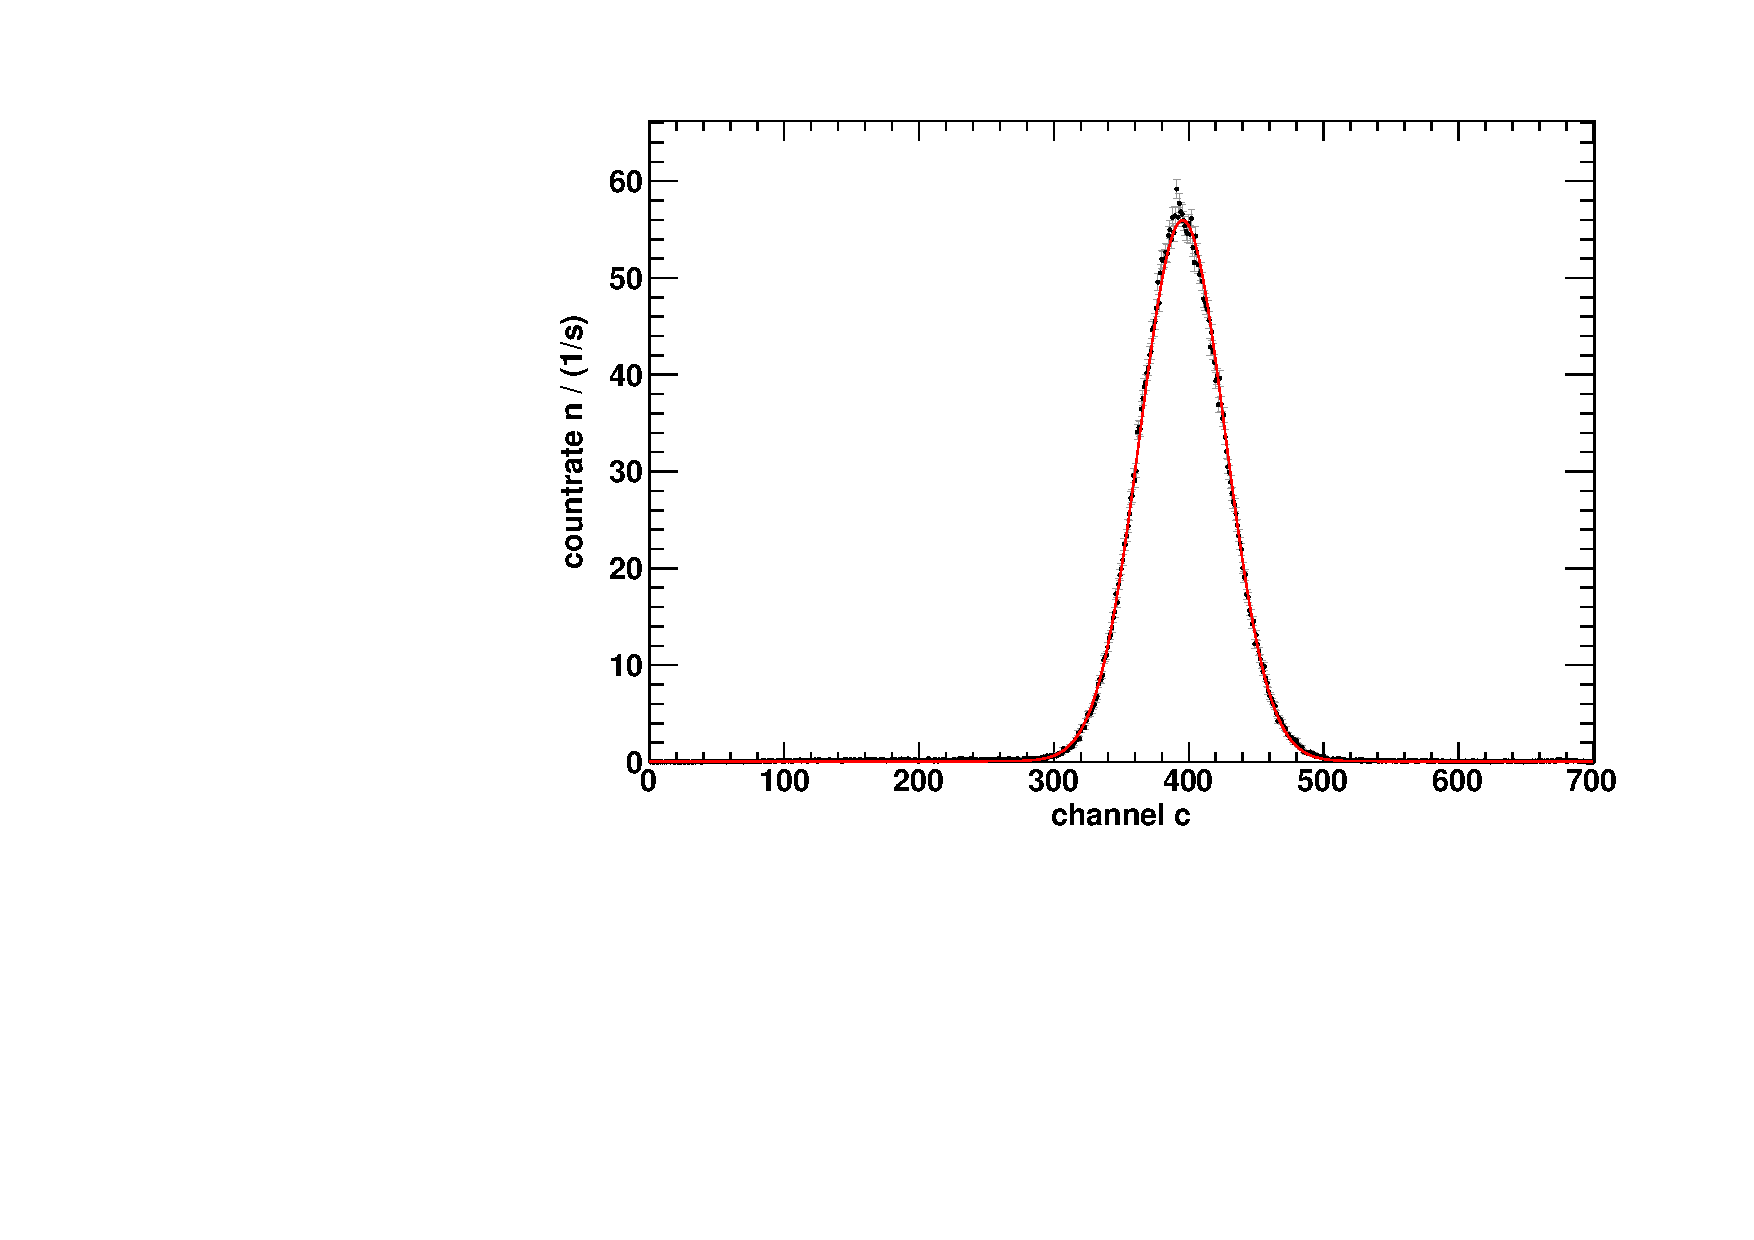
\includegraphics[width=\textwidth]{../img/energieaufloesung_400.pdf}
  \caption{Recorded and fitted spectrum of the LED flashing in the tank for one minute with medium intensity.}
  \label{img:eres:400}
\end{center}
\end{figure}

\begin{figure}[H]
\begin{center}
  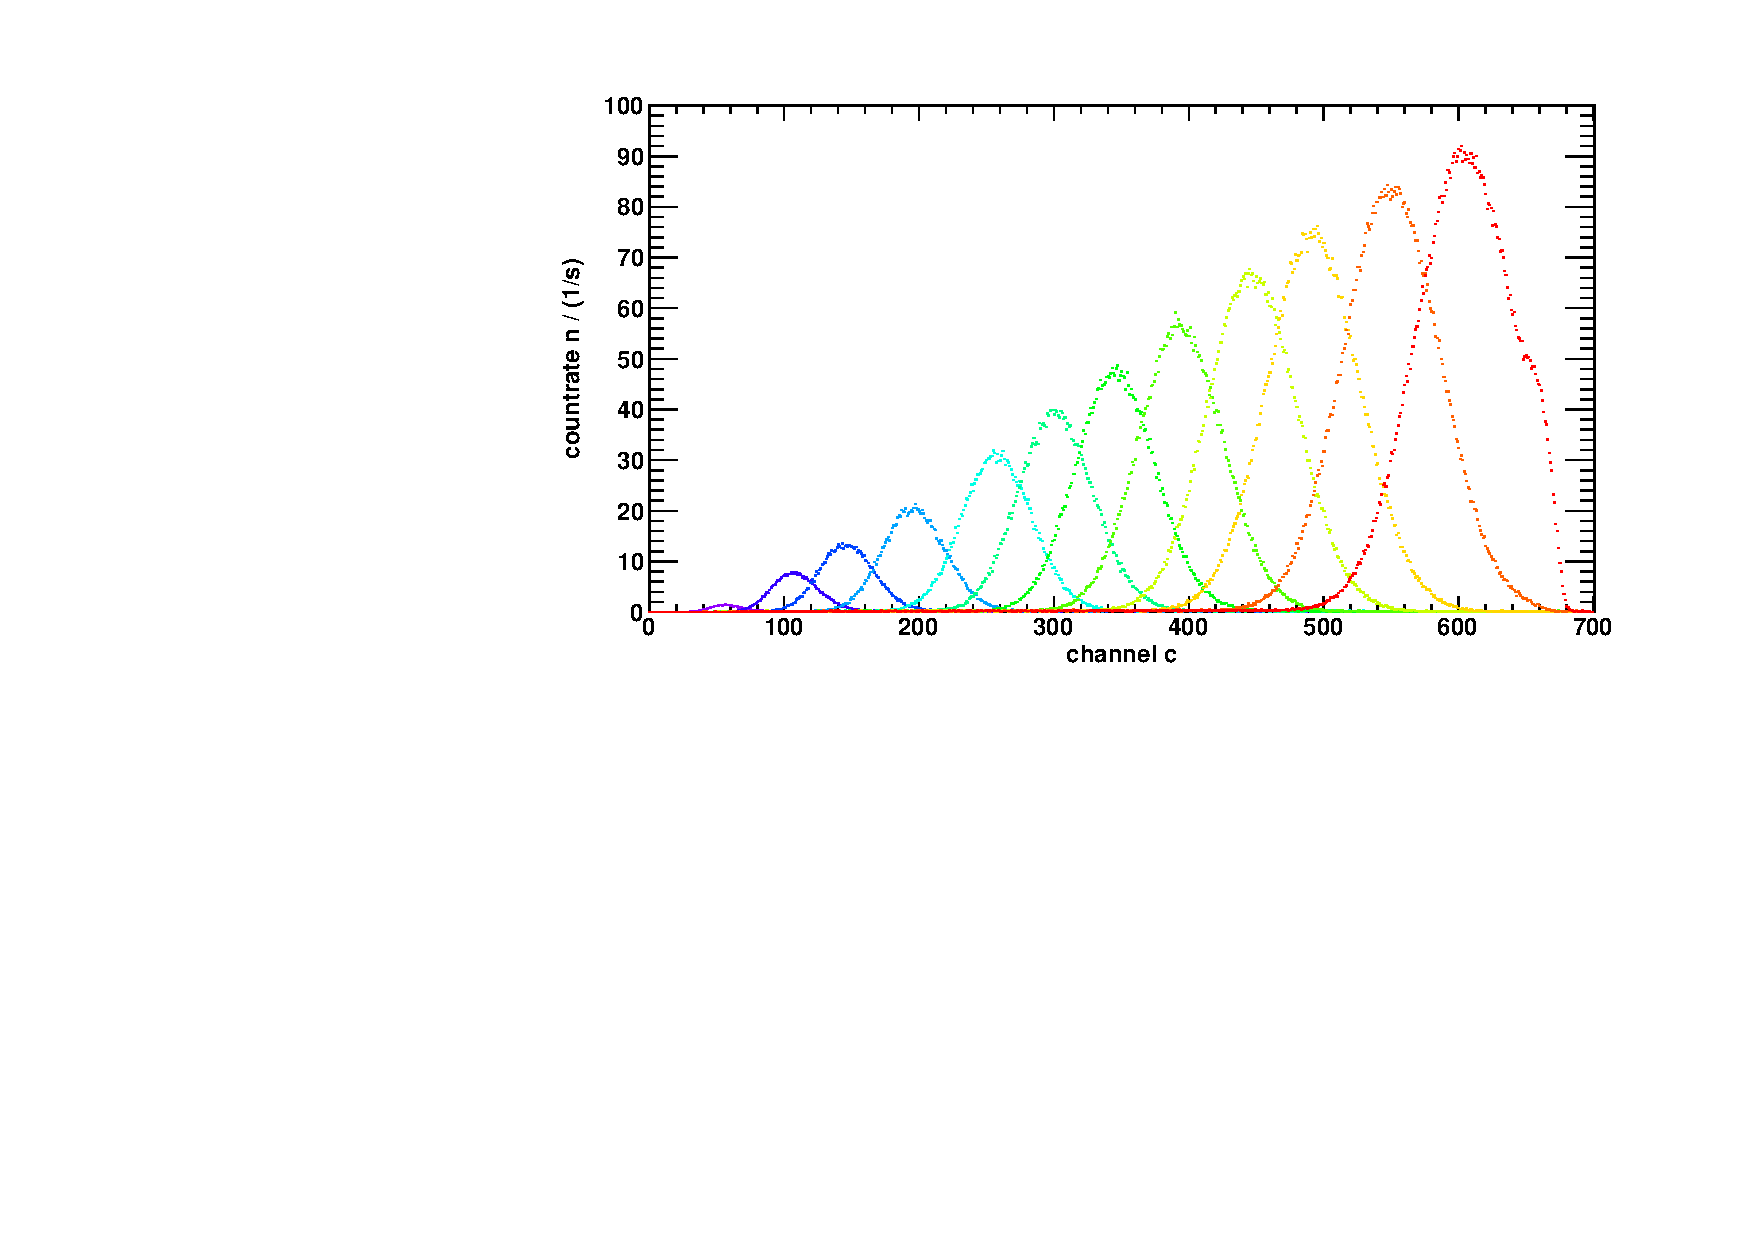
\includegraphics[width=\textwidth]{../img/energieaufloesung_multi.pdf}
  \caption{All measured energy spectra of the flashing LED in the tank.
  Raising the intensity of the LED increases the expectation value,
  the standard deviation (energy uncertainty) and the amplitude of the distributions.}
  \label{img:eres:multi}
\end{center}
\end{figure}


\begin{figure}[H]
\begin{center}
  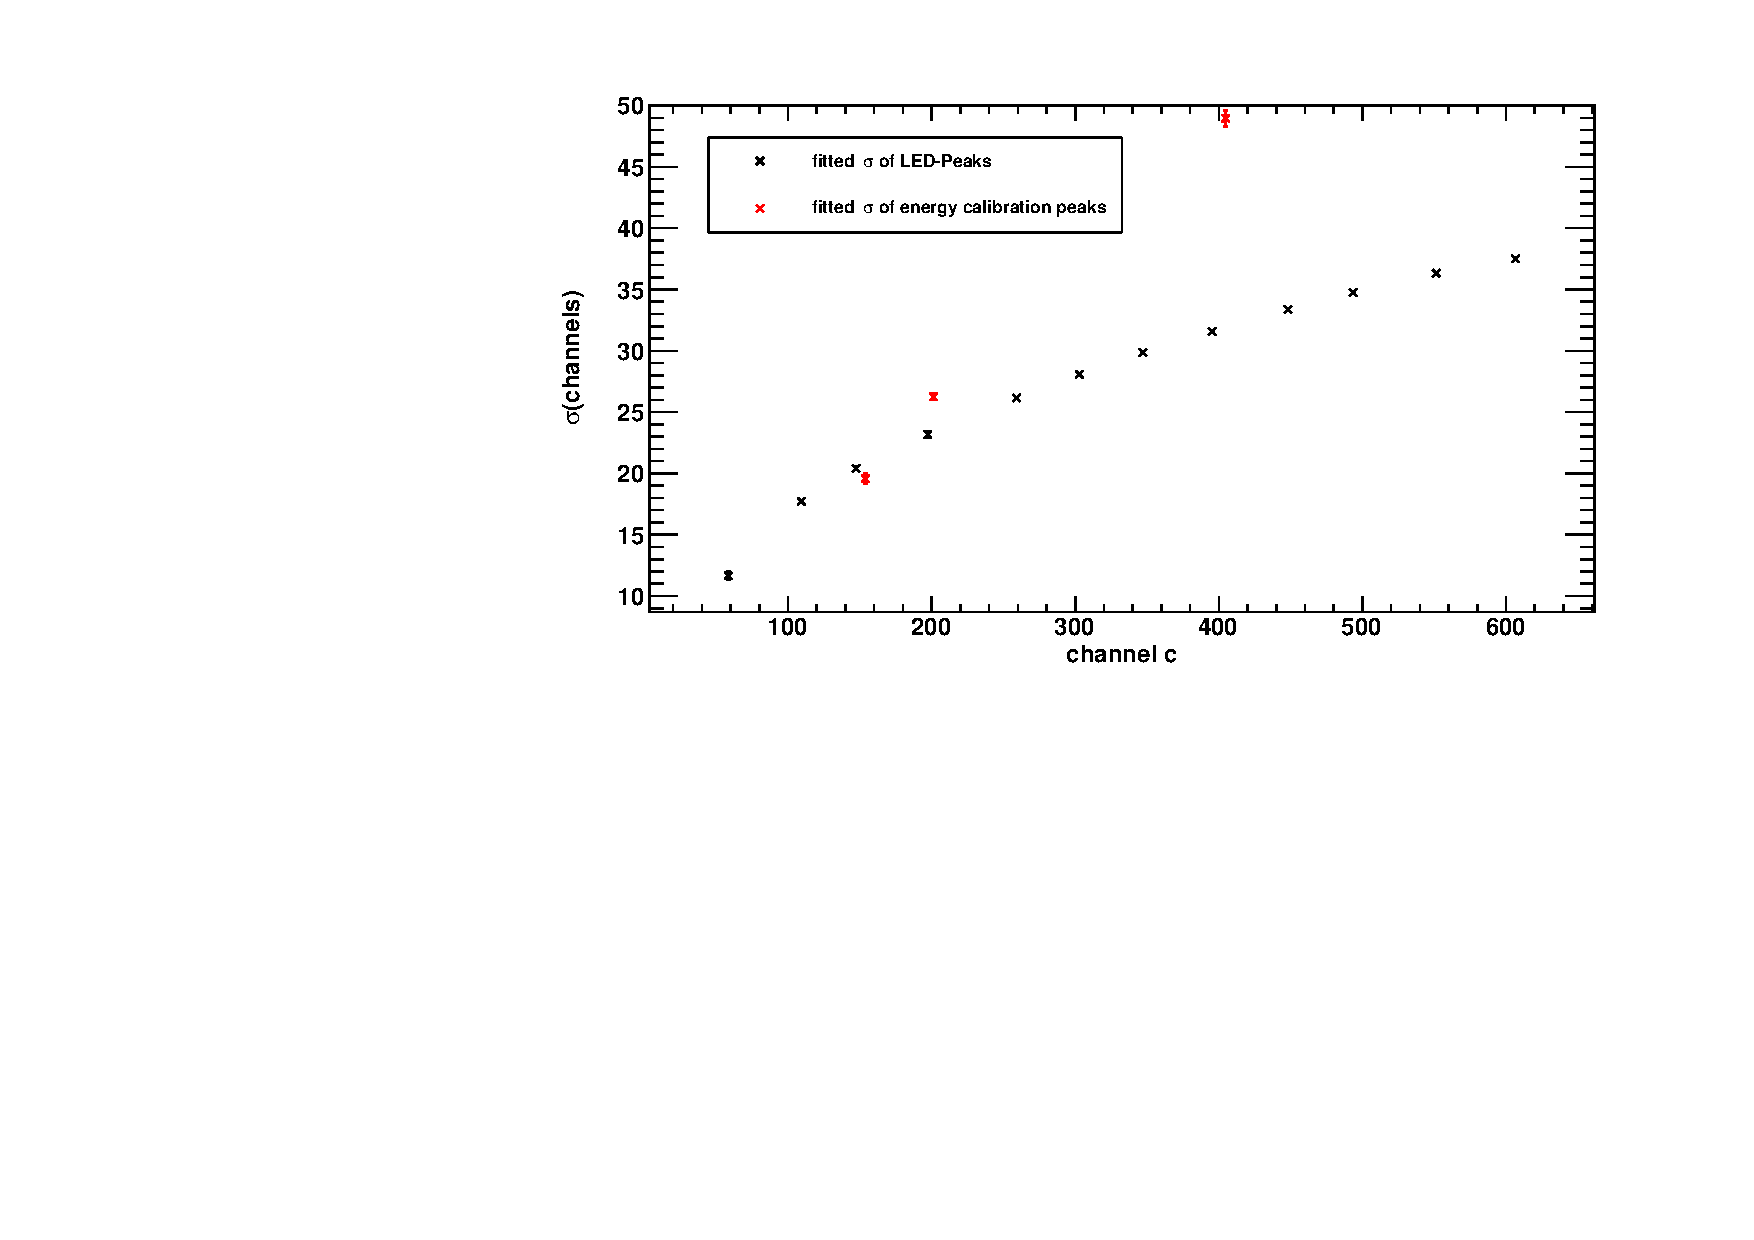
\includegraphics[width=\textwidth]{../img/energieaufloesung_channels+ecal.pdf}
  \caption{Fitted standard deviations plotted against the expectation value of their respective Gaussian distributions as seen in 
  \autoref{img:eres:multi}. The red points are the blurs of the flight through spectra (evaluated in section \ref{subsub:flightthroughspectra}).}
  \label{img:eres:channels}
\end{center}
\end{figure}

\subsection{Energy calibration}
For the energy calibration the pedestal measurement and flight through spectra are evaluated. Then the theoretical energies are calculated 
and those two datasets are plotted against each other.
\subsubsection{Pedestal}
The pedestal measurement produced a Gaussian distributed spectrum (\autoref{img:pedestal}).
\begin{figure}[H]
\begin{center}
  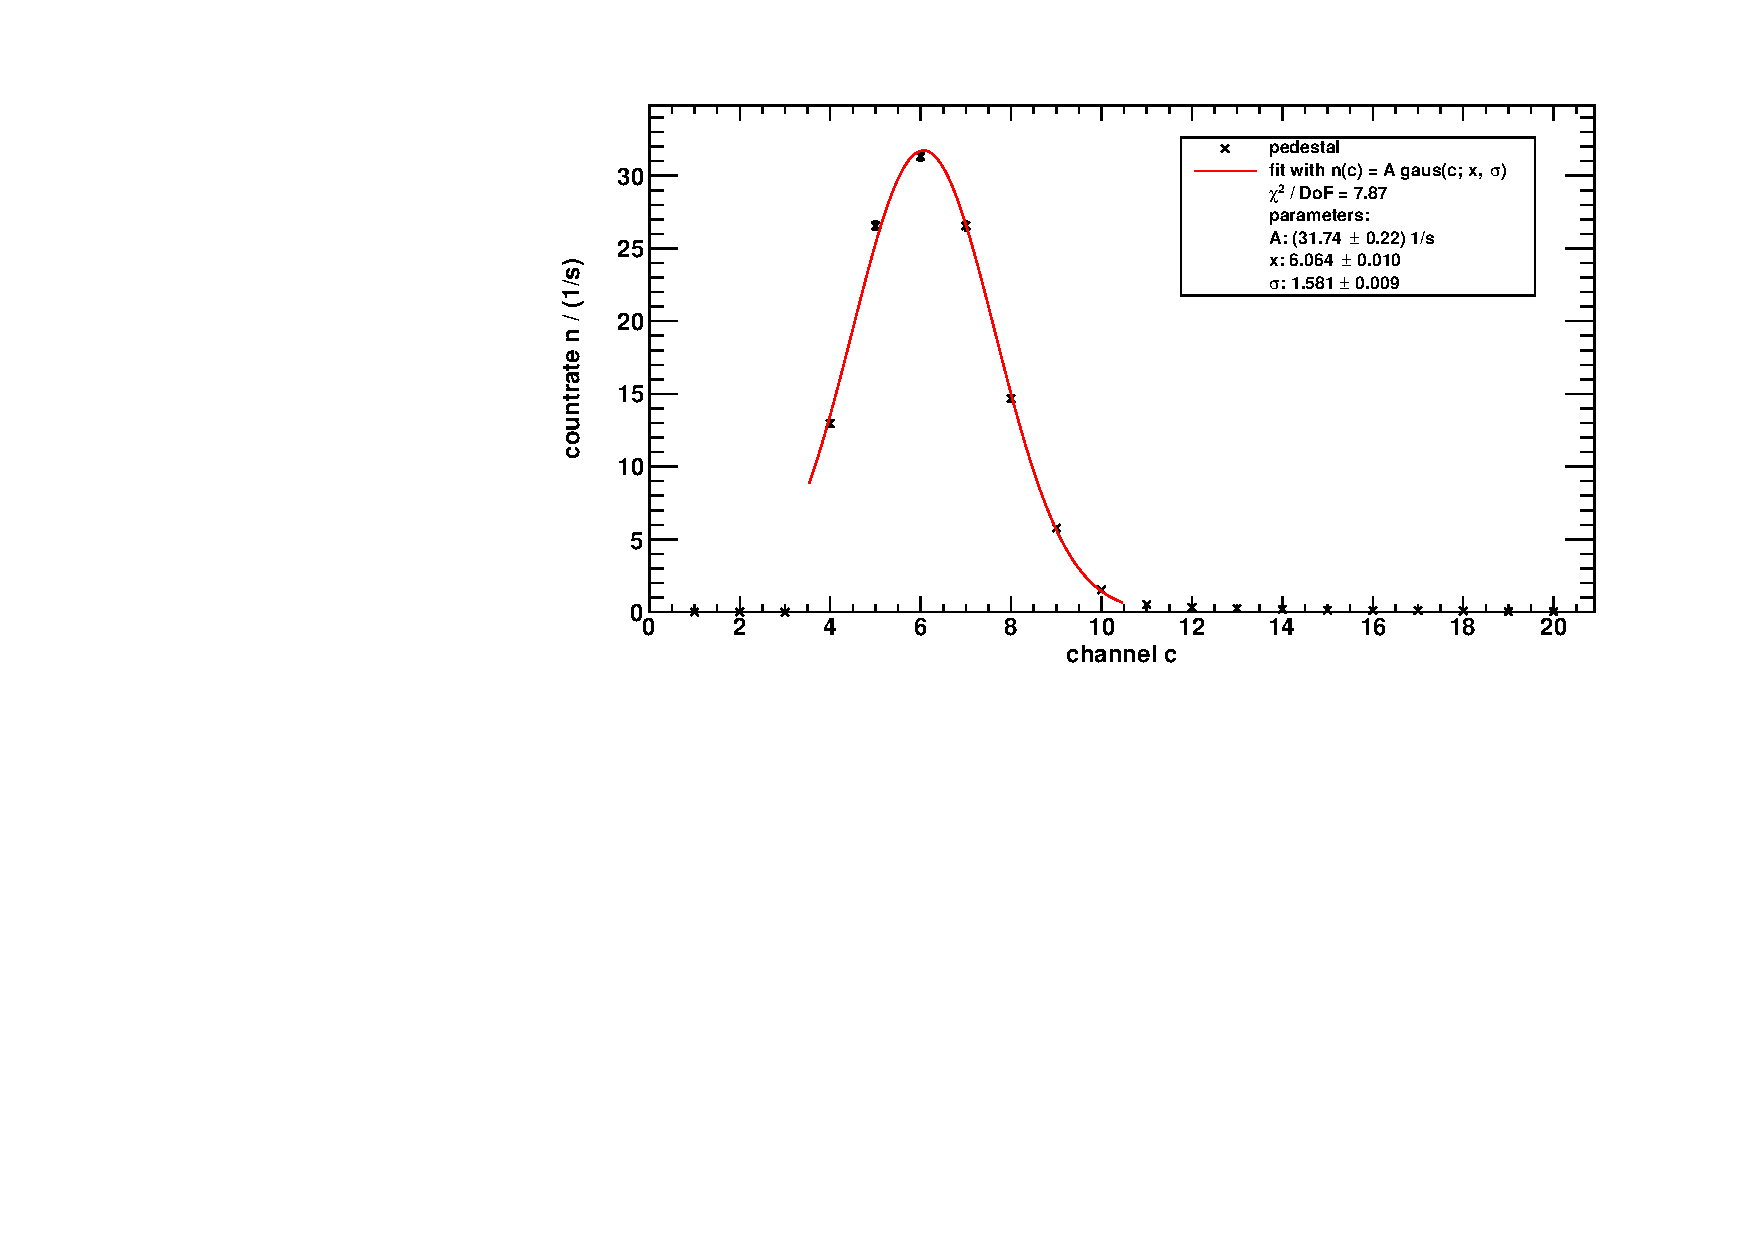
\includegraphics[width=\textwidth]{../img/pedestal.pdf}
  \caption{Pedestal: Peak at the low end of the energy spectrum caused by opening the linear gate without the occurrence of a passing signal. 
  The reason for the pedestal is shown in \autoref{img:delcapgate}.}
  \label{img:pedestal}
\end{center}
\end{figure}
The peak is fitted with the Gaussian distribution multiplied by an amplitude $A$:
\begin{equation}
    n(c) = A \cdot \gaus(c;x,\sigma)
\end{equation}
The expectation value of the fitted Gaussian distribution is:
\begin{equation}
    x = (6.064 \pm 0.010)
\end{equation}

\subsubsection{Flight through spectra}
\label{subsub:flightthroughspectra}
\paragraph{Landau distribution}
The Landau distribution describes the fluctuations of energy loss caused by impact 
ionization\footnote{The distribution follows from the \emph{Bethe formula}.}.
But the measured data is not described by just a Landau distribution, since the spectrum is blurred by the energy resolution of the scintillator. 
To get a function for fitting a convolution of the Landau distribution with a Gaussian distribution is needed:
\begin{equation}
    \label{eq:landaugausconv}
    (\landau(\mu, s) *  \gaus(0, \sigma))(c) = \int_{-\infty}^{\infty} \landau(x;\mu, s) \gaus(c-x;0,\sigma)\difd x
\end{equation}
Since there is no analytical closed form for the Landau distribution the convolution can not be solved analytical. The spectra are fitted with a
numerical convolution\footnote{The code is based on \url{https://root.cern.ch/root/html/tutorials/fit/langaus.C.html}, translated to Python by us.}. 
The spectra with their fits are shown in \autoref{img:ecal:100}, \autoref{img:ecal:50} and \autoref{img:ecal:35}. The fitted parameters are listed in 
\autoref{tab:ecal}.
\begin{figure}[H]
\begin{center}
  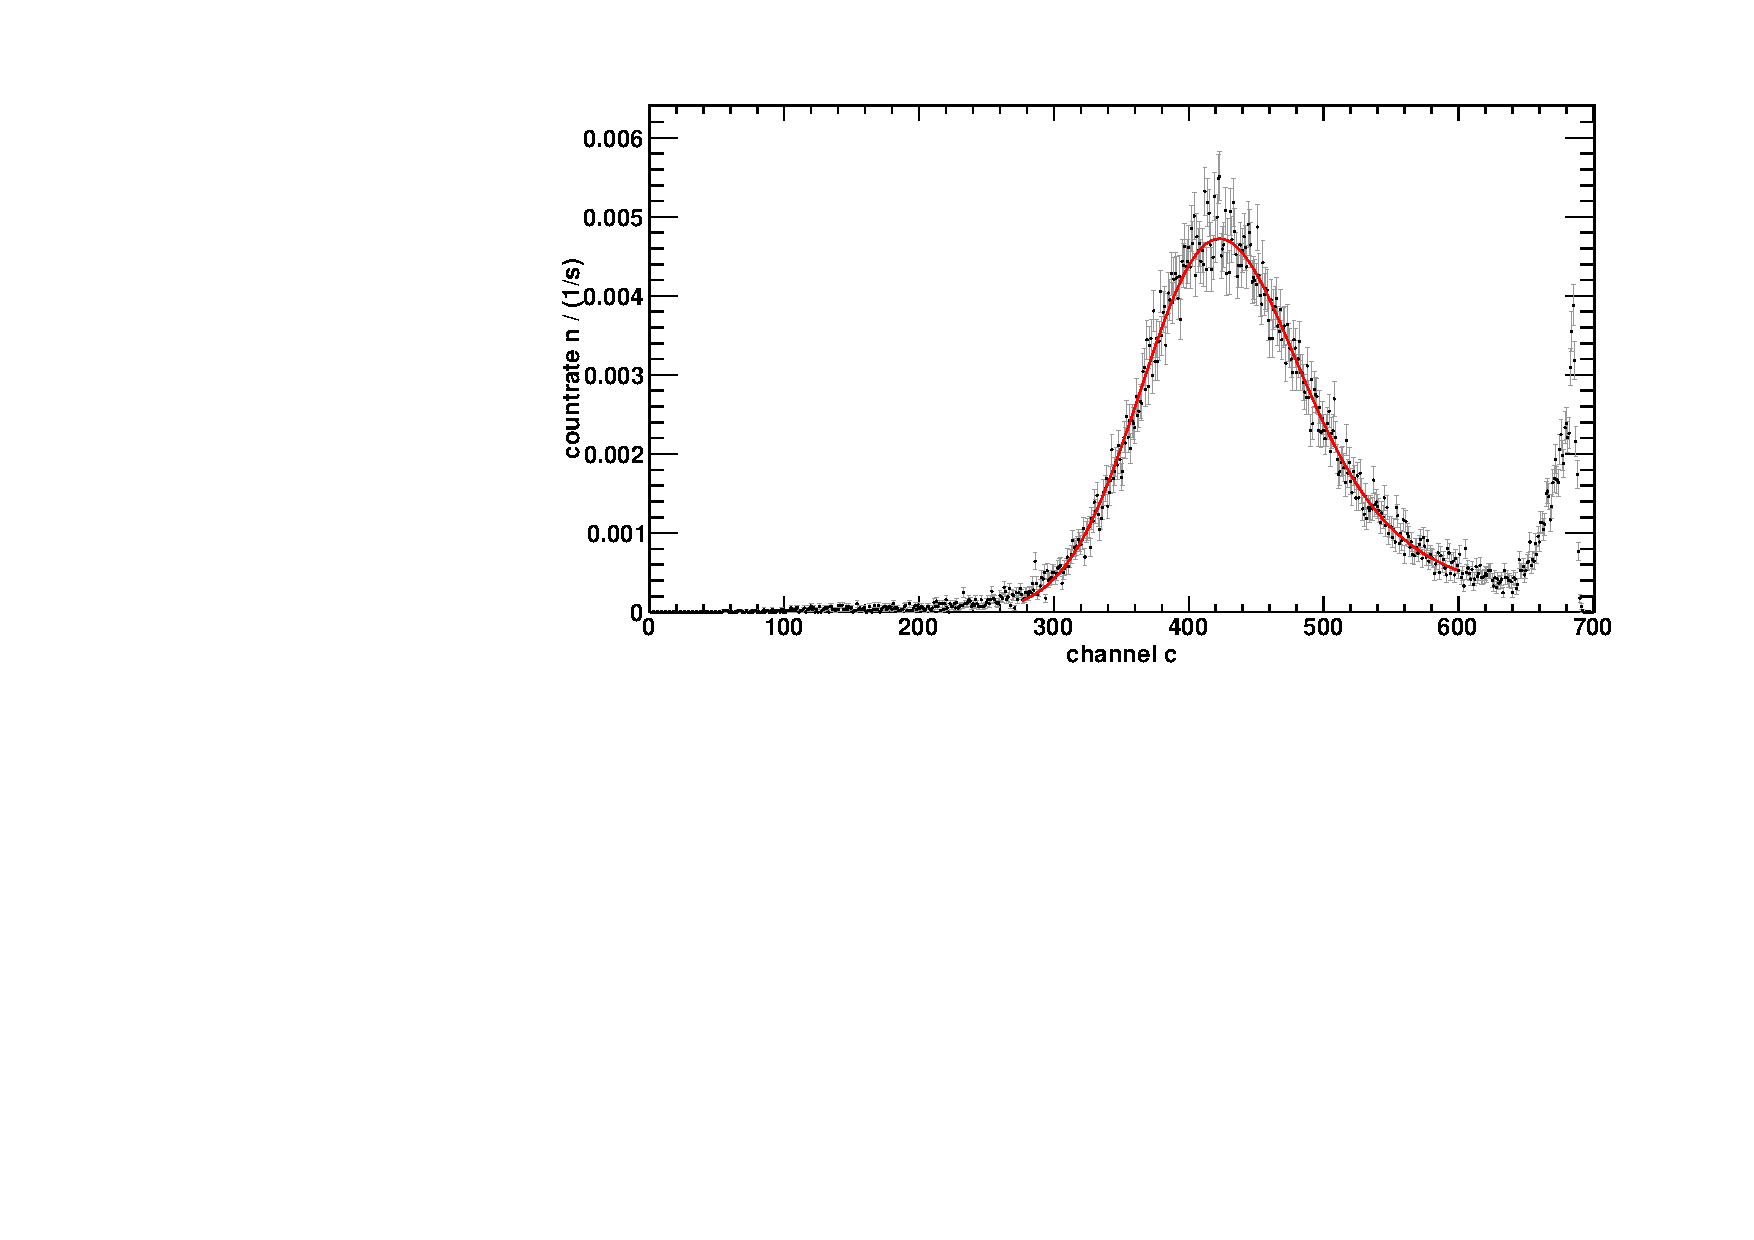
\includegraphics[width=\textwidth]{../img/energiekalibration_100.pdf}
  \caption{Flight through spectrum of muons with 12\,dB attenuation ($\overset{\wedge}{=}$ 100\% energy) with a blurred Landau fit.}
  \label{img:ecal:100}
\end{center}
\end{figure}

\begin{figure}[H]
\begin{center}
  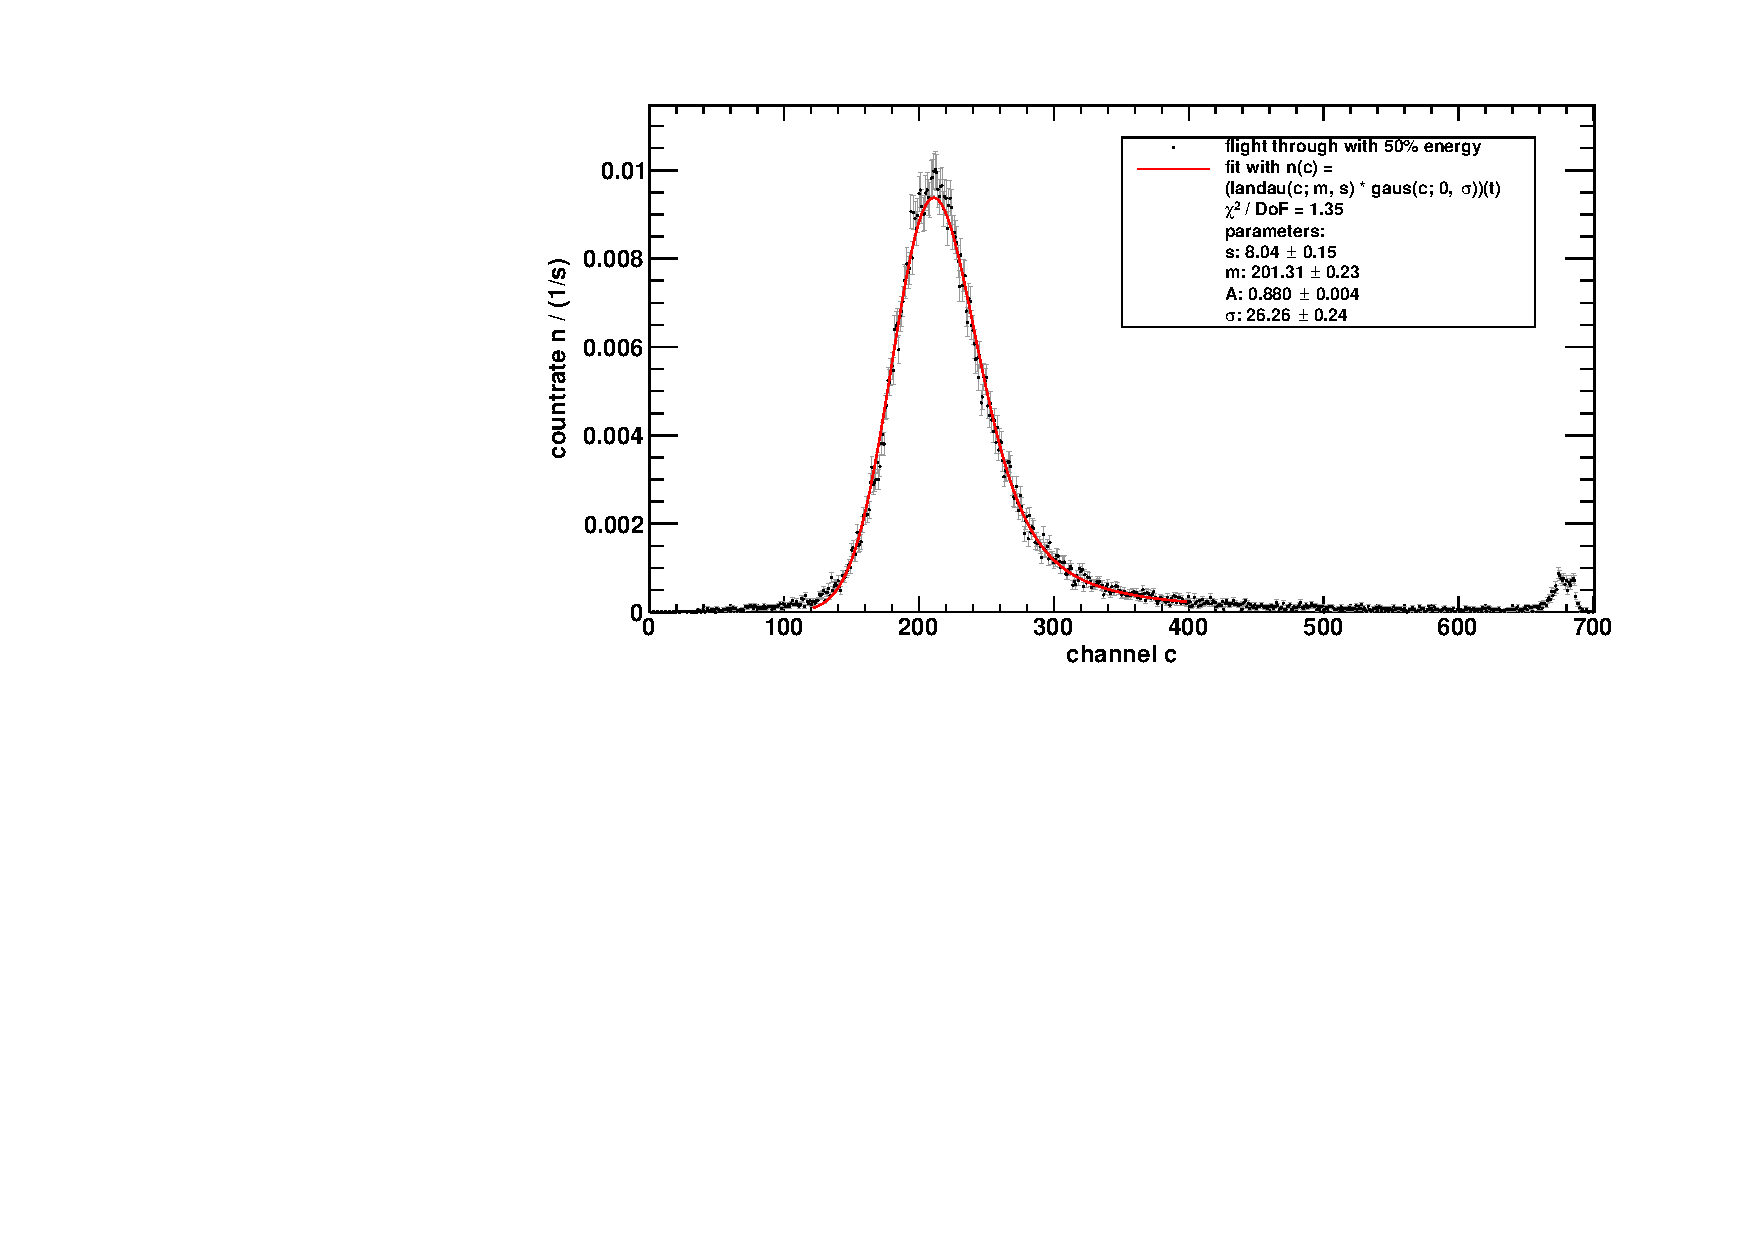
\includegraphics[width=\textwidth]{../img/energiekalibration_50.pdf}
  \caption{Flight through spectrum of muons with 18\,dB attenuation ($\overset{\wedge}{=}$ 50\% energy) with a blurred Landau fit.}
  \label{img:ecal:50}
\end{center}
\end{figure}

\begin{figure}[H]
\begin{center}
  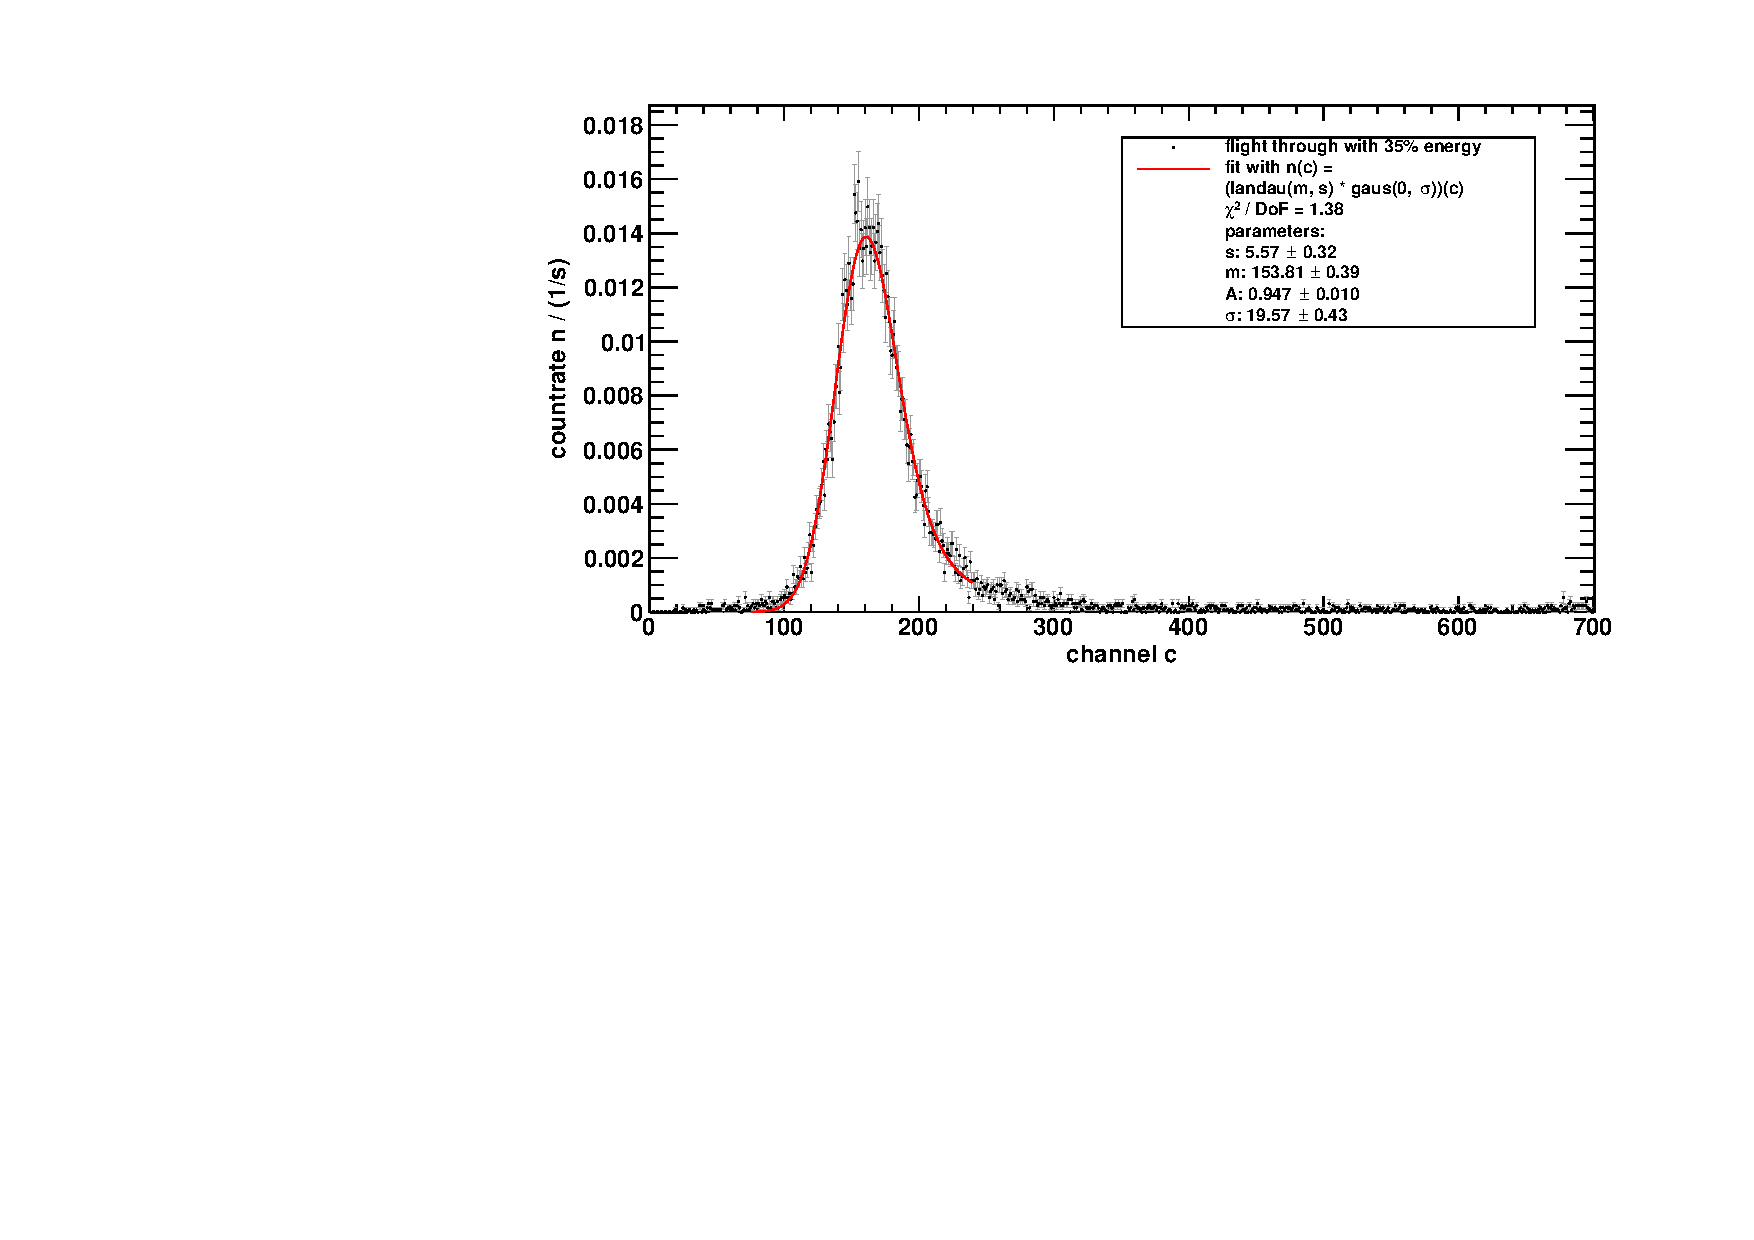
\includegraphics[width=\textwidth]{../img/energiekalibration_35.pdf}
  \caption{Flight through spectrum of muons with 21\,dB attenuation ($\overset{\wedge}{=}$ 35\% energy) with a blurred Landau fit.}
  \label{img:ecal:35}
\end{center}
\end{figure}

\subsubsection{Verification of the attenuator}
The measured amplitudes $A$ of the attenuated signals are shown in \autoref{tab:attenuator}.
\begin{table}[H]
\caption{Measured amplitude $A$ of a periodic rectangular signal after the attenuation with nominal value $n$.}
\begin{center}
\begin{tabular}{|c|c|c|}
    \hline
    $n$ / dB 	& $A$ / mV 	& $s_A$ / mV	\\ \hline \hline
    0 			& 840		& 40			\\ \hline
    12			& 210		& 10			\\ \hline
    18			& 106		& 4				\\ \hline
    21			& 75		& 4				\\ \hline
\end{tabular}
\end{center}
\label{tab:attenuator}
\end{table}
The measured attenuation $m$ can be calculated with
\begin{equation}
    m = - 20 \log_{10} \left( \frac{A}{A_0} \right), \qquad s_m = \frac{20}{\ln 10} \sqrt{ \left( \frac{s_A}{A} \right)^2 + \left( \frac{s_{A_0}}{A_0} \right)^2}
\end{equation}
where $A_0$ is the the amplitude at $n=0$\,dB.
Those attenuations can be plotted against the nominal values (\autoref{img:attenuator}).
\begin{figure}[H]
\begin{center}
  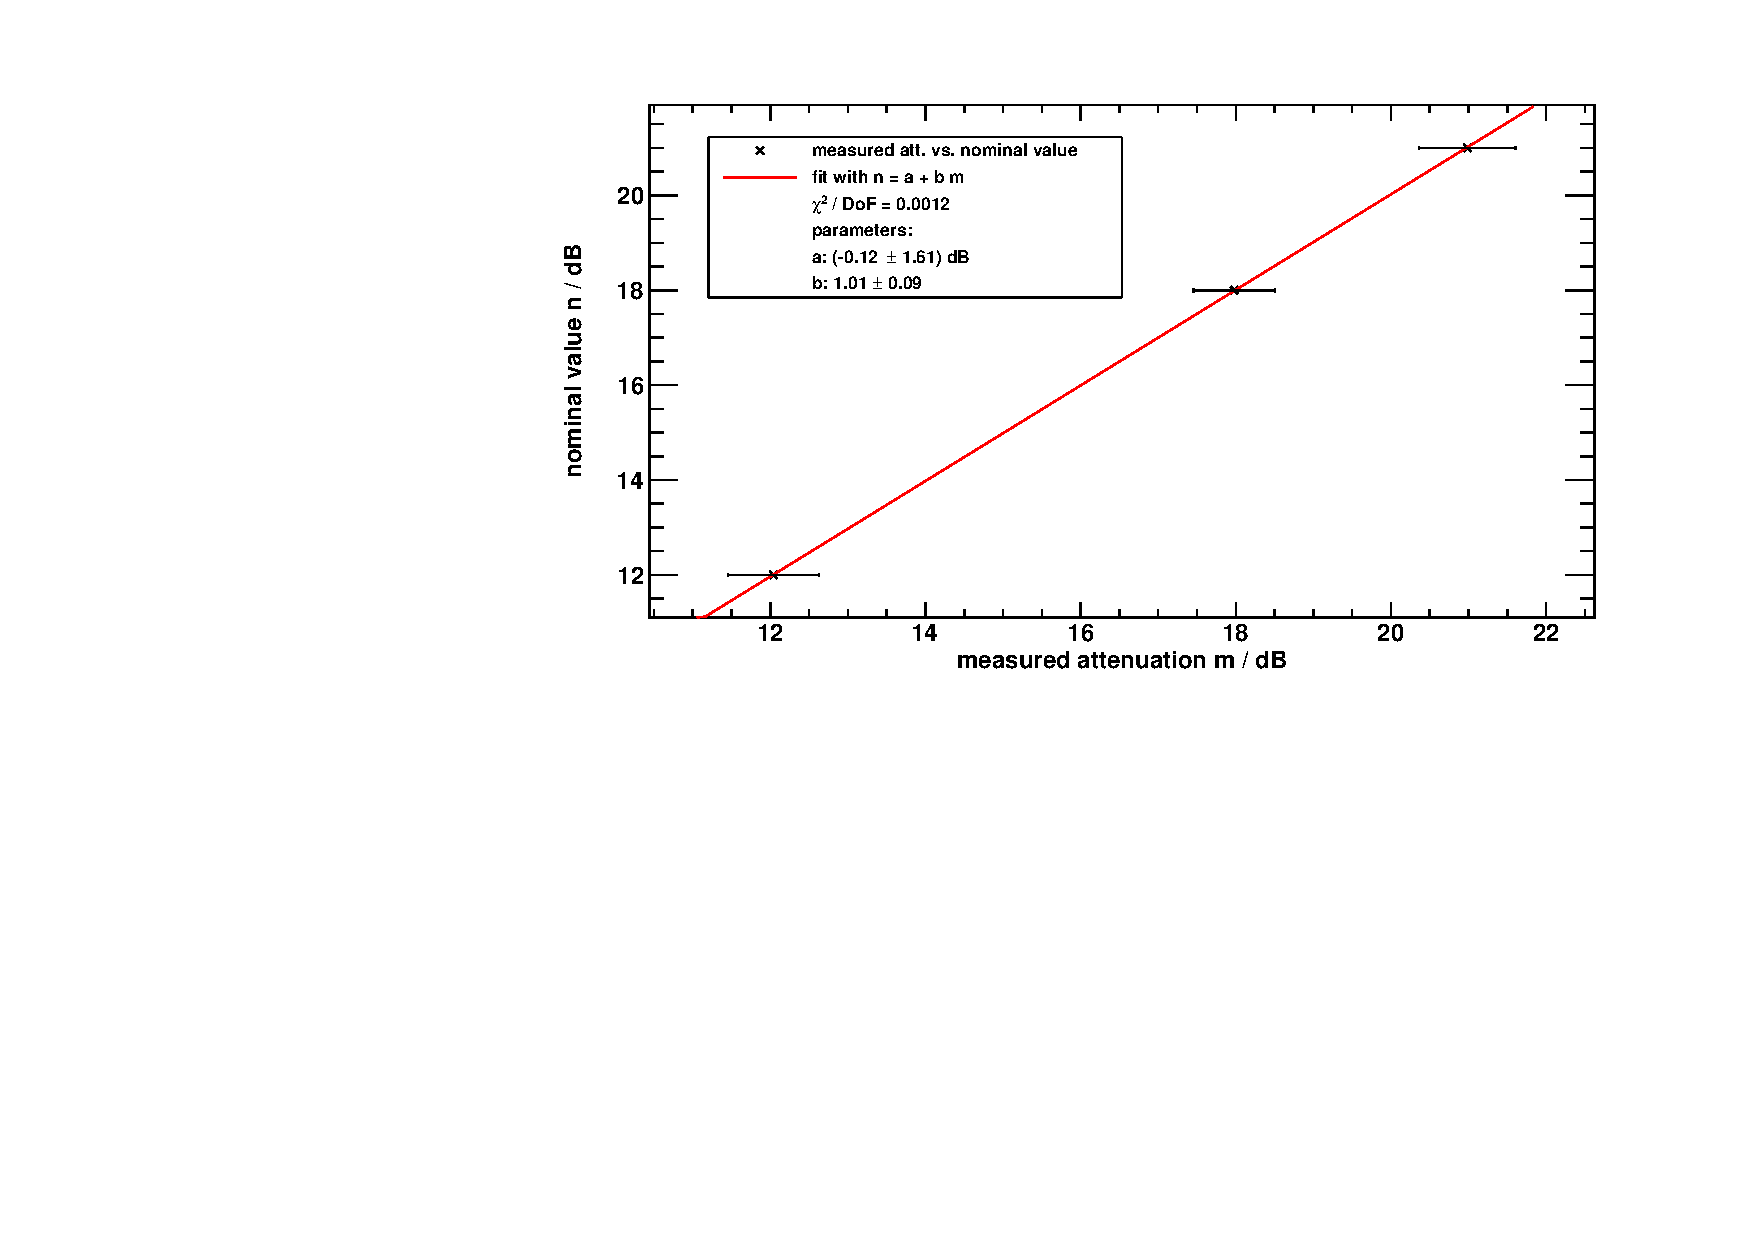
\includegraphics[width=\textwidth]{../img/attenuator.pdf}
  \caption{Nominal attenuations $n$ plotted against the measured attenuations $m$ and fit with a line.}
  \label{img:attenuator}
\end{center}
\end{figure}
If the attenuator works correctly, the linear fit should yield a line with intercept $a=0$\,dB and slope $b=1$. The fit results are:
\begin{equation}
    \begin{split}
        & a = (-0.1 \pm 1.6)\,\text{dB} \\
        & b = 1.01  \pm 0.09 
    \end{split}
\end{equation}
Therefore we conclude that the attenuator works correctly and no correction is needed.

\subsubsection{Calibration}
For the calibration it must be known how much energy a muon deposits in the tank. Following data was given:
\begin{equation}
    \begin{split}
        & \frac{\partial E}{\partial \rho x} = (1.95 \pm 0.05)\,\frac{\text{MeV}\cdot\text{cm}^2}{\text{g}} \qquad \text{(minimal ionizing muon)}  \\
        & \rho = (0.87 \pm 0.01) \, \frac{\text{g}}{\text{cm}^3}  \qquad \qquad \qquad \text{(density of solvent)} \\
        & s = (84 \pm 5) \, \text{cm} \qquad \qquad \qquad \qquad \quad  \text{(mean free path in tank)}
    \end{split}
\end{equation}
Hence the total loss of energy calculates to:
\begin{equation}
    \begin{split}
        & E = \frac{\partial E}{\partial \rho x} \cdot \rho \cdot s = 142.5\,\text{MeV} \\
        & s_{E} = E \cdot \sqrt{ \left( \frac{s_{\frac{\partial E}{\partial \rho x}}}{\frac{\partial E}{\partial \rho x}} \right)^2 + \left( \frac{s_\rho}{\rho} \right)^2 + \left( \frac{s_s}{s} \right)^2  }
        = 9.4
    \end{split}
\end{equation}
The percentage loss of energy can now be determined:
\begin{equation}
    E_p = p \cdot E, \qquad s_{E_p} = p \cdot s_E, \qquad 0 \leq p \leq 1  %TODO Fehler auf p wegen Dämpfer?
\end{equation}
The fitted peaks of the energy calibration and their respective energies are listed in \autoref{tab:ecal} and visualized in \autoref{img:energycalibration}.
\begin{table}[H]
\caption{Channels of fitted peaks and their theoretical energy for the energy calibration.}
\begin{center}
\begin{tabular}{|c|c|c|c|c|}
  \hline
  \% energy & $c$ & $s_c$ & $E$ / MeV & $s_E$ / MeV \\ \hline
  0 & 6.064 & 0.010 & 0.0 & 0.0 \\ \hline
  35 & 153.808 & 0.392 & 49.9 & 3.0 \\ \hline
  50 & 201.312 & 0.225 & 71.3 & 4.3 \\ \hline
  100 & 404.770 & 0.547 & 142.5 & 8.5 \\ \hline
\end{tabular}
\end{center}
\label{tab:ecal}
\end{table}

\begin{figure}[H]
\begin{center}
  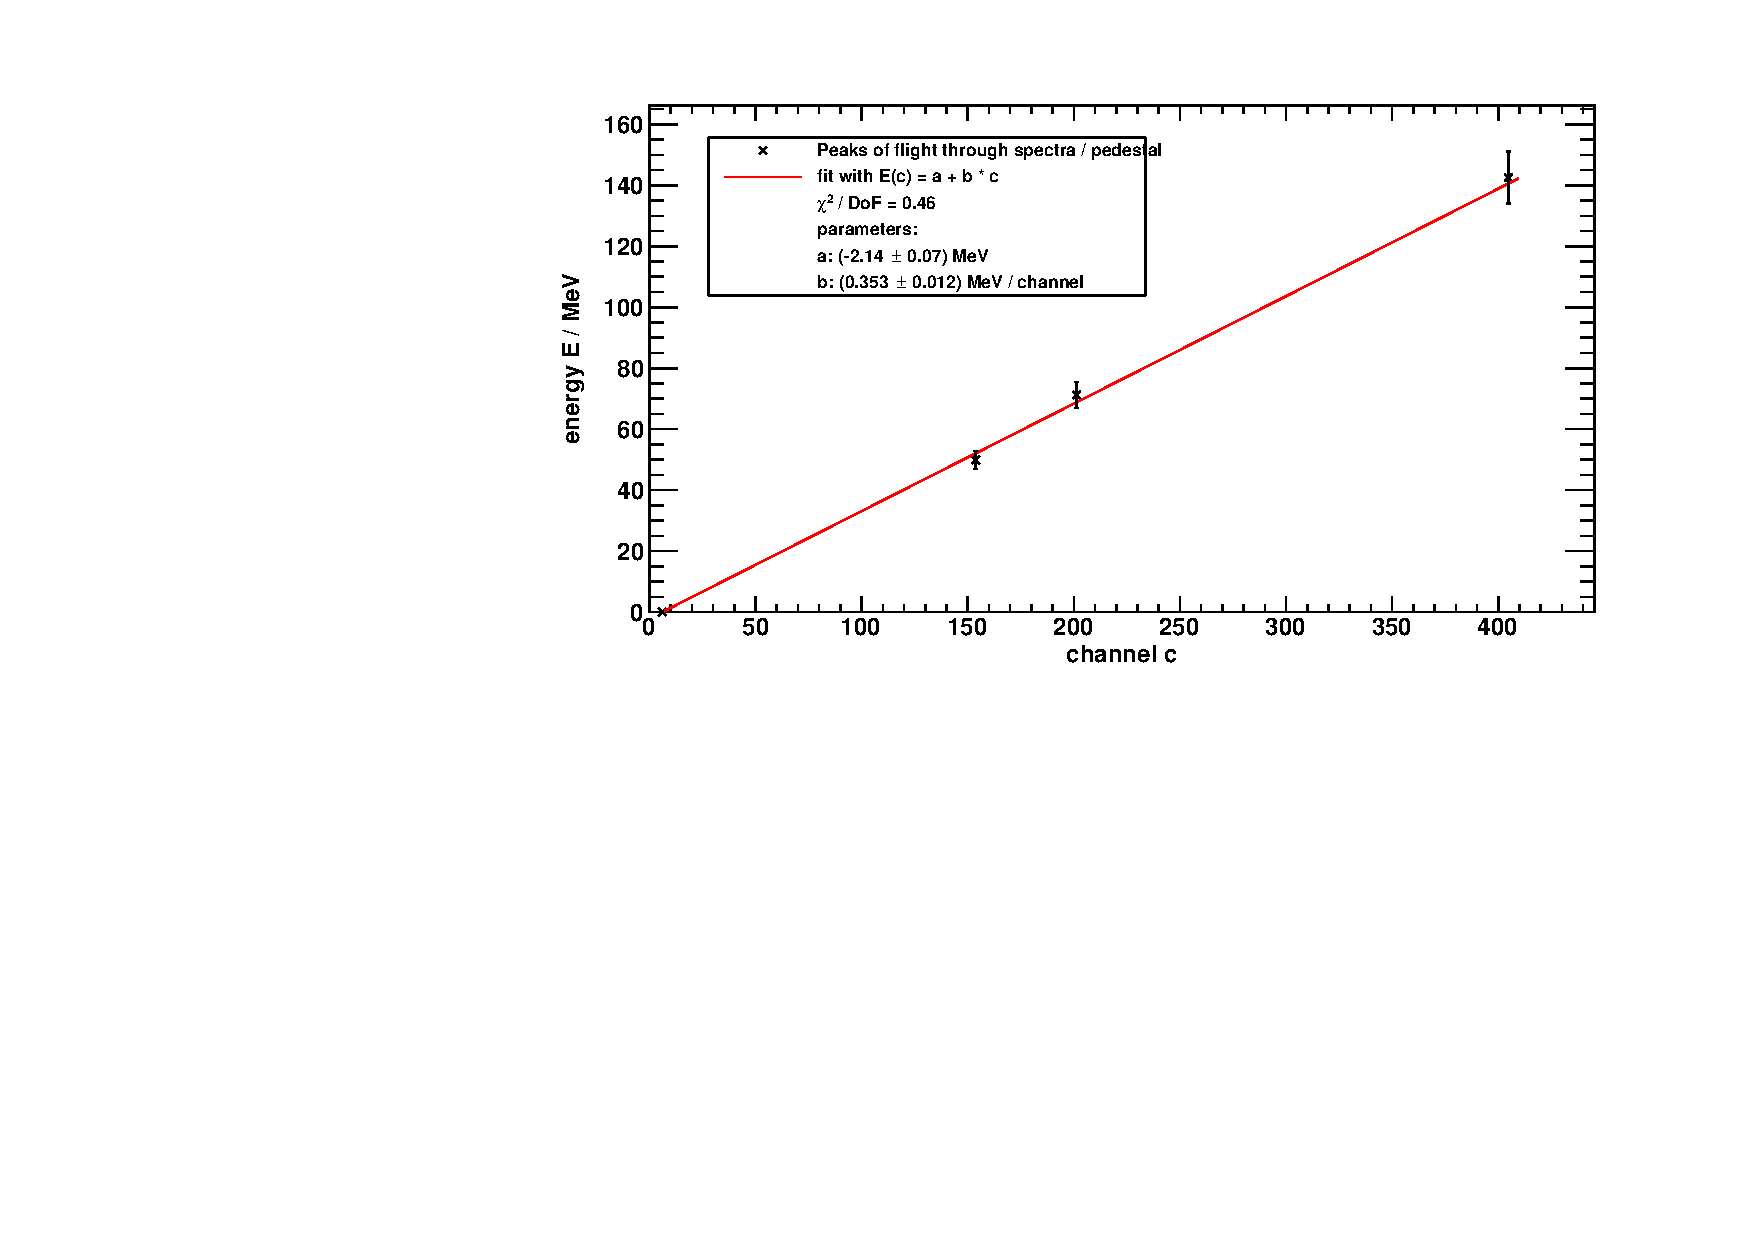
\includegraphics[width=\textwidth]{../img/energyCalibration.pdf}
  \caption{Energy calibration.}
  \label{img:energycalibration}
\end{center}
\end{figure}
Since the scintillators should produce a signal amplitude linear to the measured energy, a linear fit is implemented:
\begin{equation}
    E(c) = a + b \cdot c
\end{equation}
The fit yields:
\begin{equation}
    \begin{split}
        & a = (-2.14 \pm 0.07) \, \text{MeV} \\
        & b = (0.353 \pm 0.012) \, \frac{\text{MeV}}{\text{channel}} \\
        & \cov(a, b) = -0.0009 \, \frac{\text{MeV}^2}{\text{channel}} 
    \end{split}
\end{equation}
Now the energy $E$ of a channel $c$ and its error $s_E$ can be calculated with:
\begin{equation}
\label{eq:ecalibration}
    E = a + b \cdot c, \qquad s_E = \sqrt{s_a^2 + \left(c \cdot s_b \right)^2 + 2 \cdot c \cdot \cov(a,b)}
\end{equation}

\subsection{Time calibration}
In \autoref{tab:tcal} the data for the time calibration is listed.
In each of the four measurements, there were only one or two channels of MCA\,II responding,
so there is no need to fit the data.
\begin{table}[H]
\caption{Measured times and channels with errors for the time calibration.}
\begin{center}
\begin{tabular}{|c|c|c|c|}
  \hline
  $t$ / \textmu s & $s_t$ / \textmu s & $c$ & $s_c$ \\ \hline
  2.40 & 0.02 & 113.0 & 0.5 \\ \hline
  4.50 & 0.02 & 223.0 & 0.5 \\ \hline
  6.25 & 0.02 & 315.5 & 0.5 \\ \hline
  8.60 & 0.02 & 441.0 & 0.5 \\ \hline
\end{tabular}
\end{center}
\label{tab:tcal}
\end{table}

A linear fit is done (\autoref{img:timecalibration}):
\begin{equation}
    t = a + b \cdot c
\end{equation}
\begin{figure}[H]
\begin{center}
  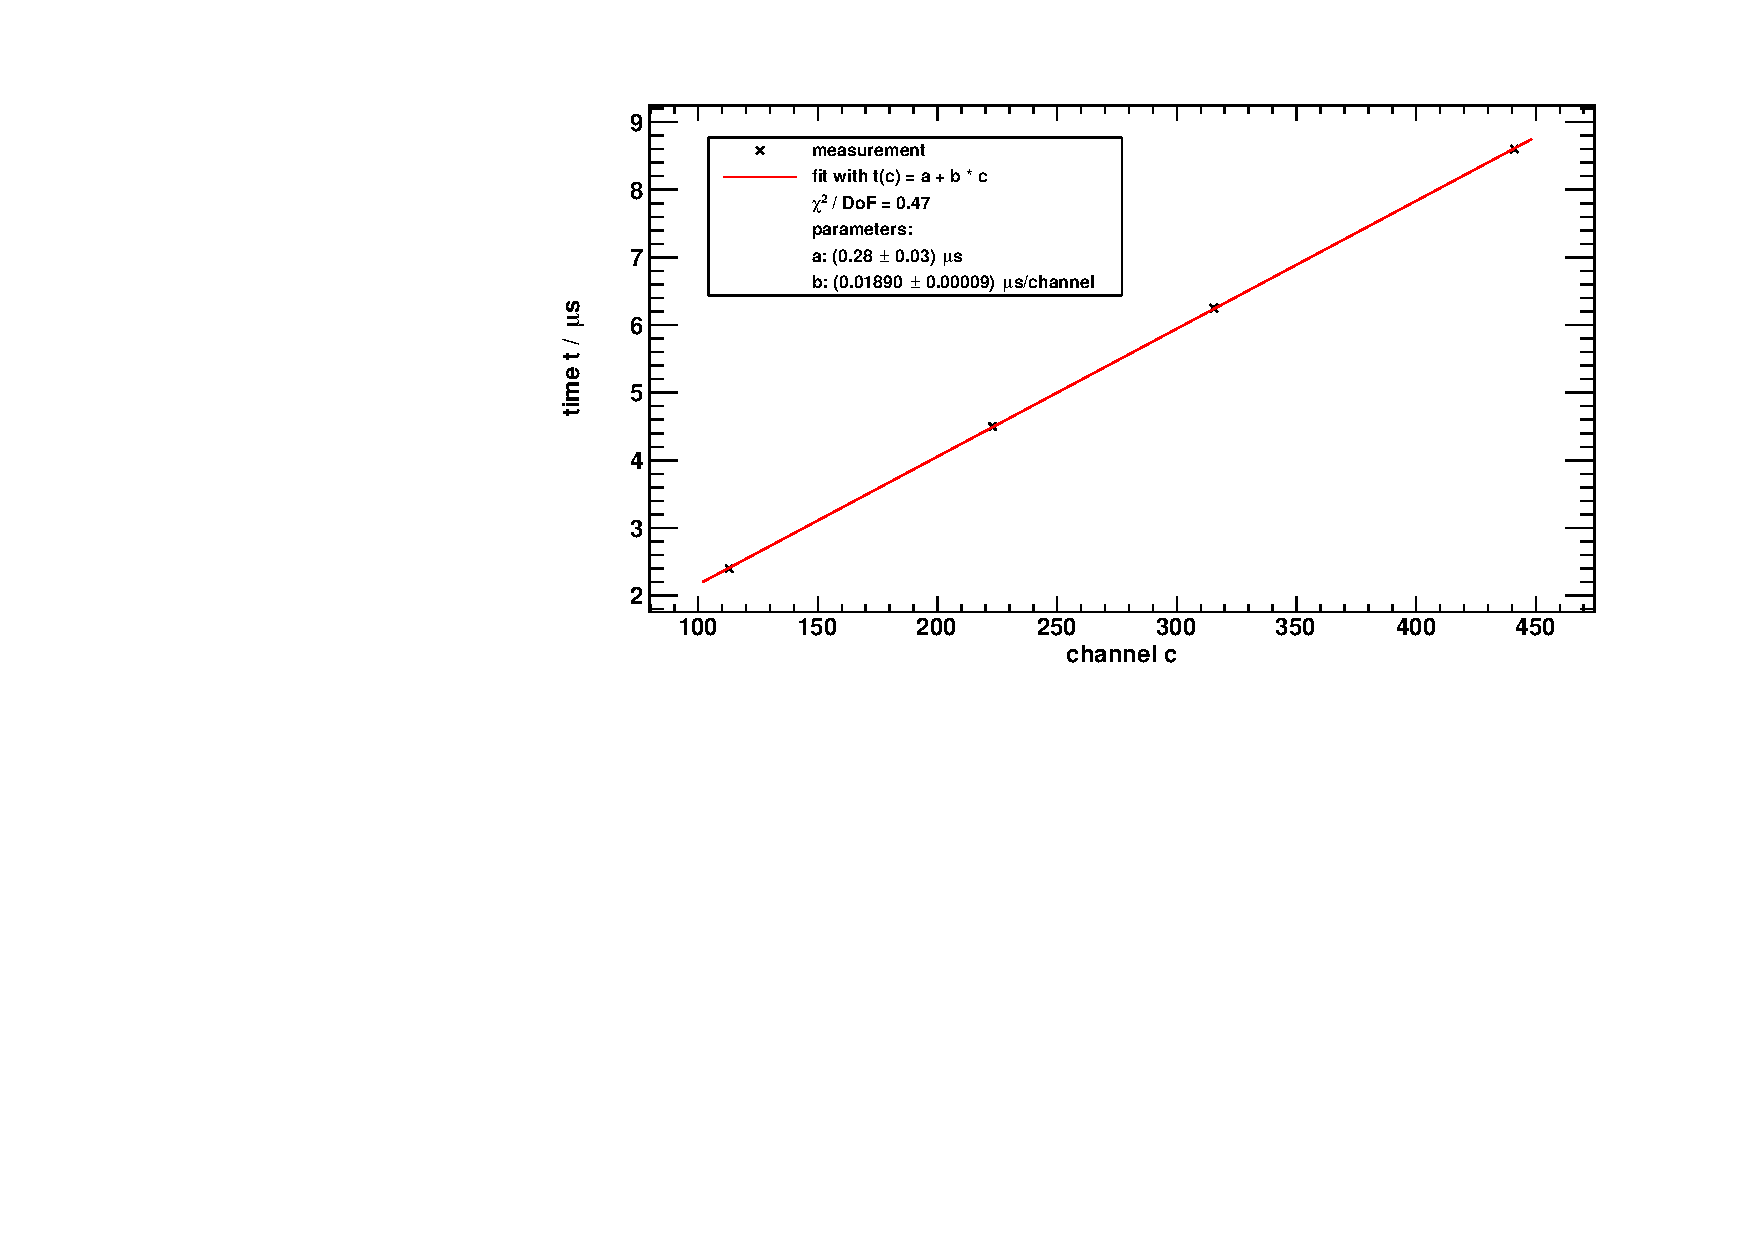
\includegraphics[width=\textwidth]{../img/timeCalibration.pdf}
  \caption{Time Calibration.}
  \label{img:timecalibration}
\end{center}
\end{figure}
The parameters and their covariance for this fit are:
\begin{equation}
    \begin{split}
        & a = (0.28 \pm 0.03) \, \text{\textmu s} \\
        & b = (0.01890 \pm 0.00009) \, \frac{\text{\textmu s}}{\text{channel}} \\
        & \cov(a, b) = -2.299 \, \frac{\text{\textmu s}^2}{\text{channel}} 
    \end{split}
\end{equation}
Now the time $t$ of a channel $c$ and its error $s_t$ can be calculated with:
\begin{equation}
\label{eq:tcalibration}
    t = a + b \cdot c, \qquad s_t = \sqrt{s_a^2 + \left(t \cdot s_b \right)^2 + 2 \cdot t \cdot \cov(a,b)}
\end{equation}

\subsection{Underground}
The underground measurement is visualized in \autoref{img:underground}.
\begin{figure}[H]
\begin{center}
  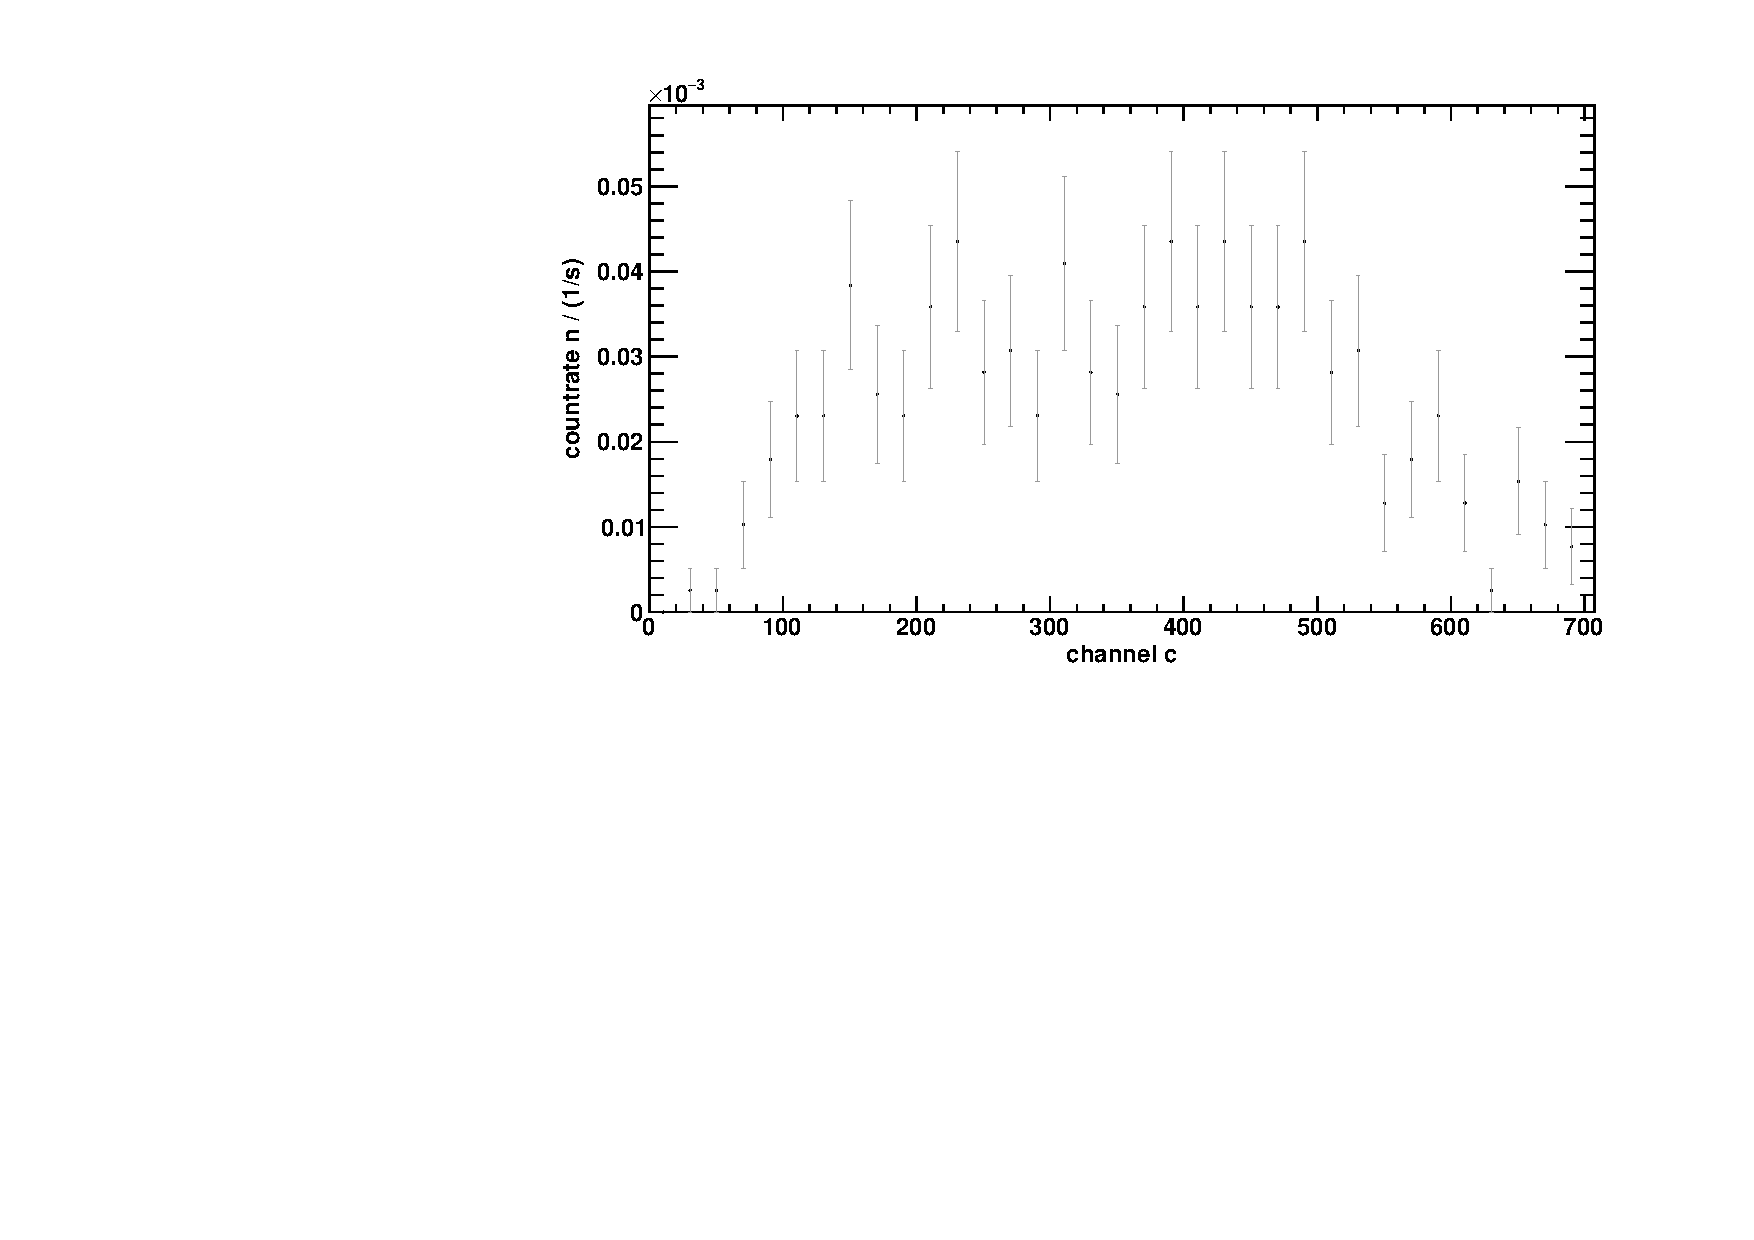
\includegraphics[width=\textwidth]{../img/underground.pdf}
  \caption{Underground.}
  \label{img:underground}
\end{center}
\end{figure}

\begin{figure}[H]
\begin{center}
  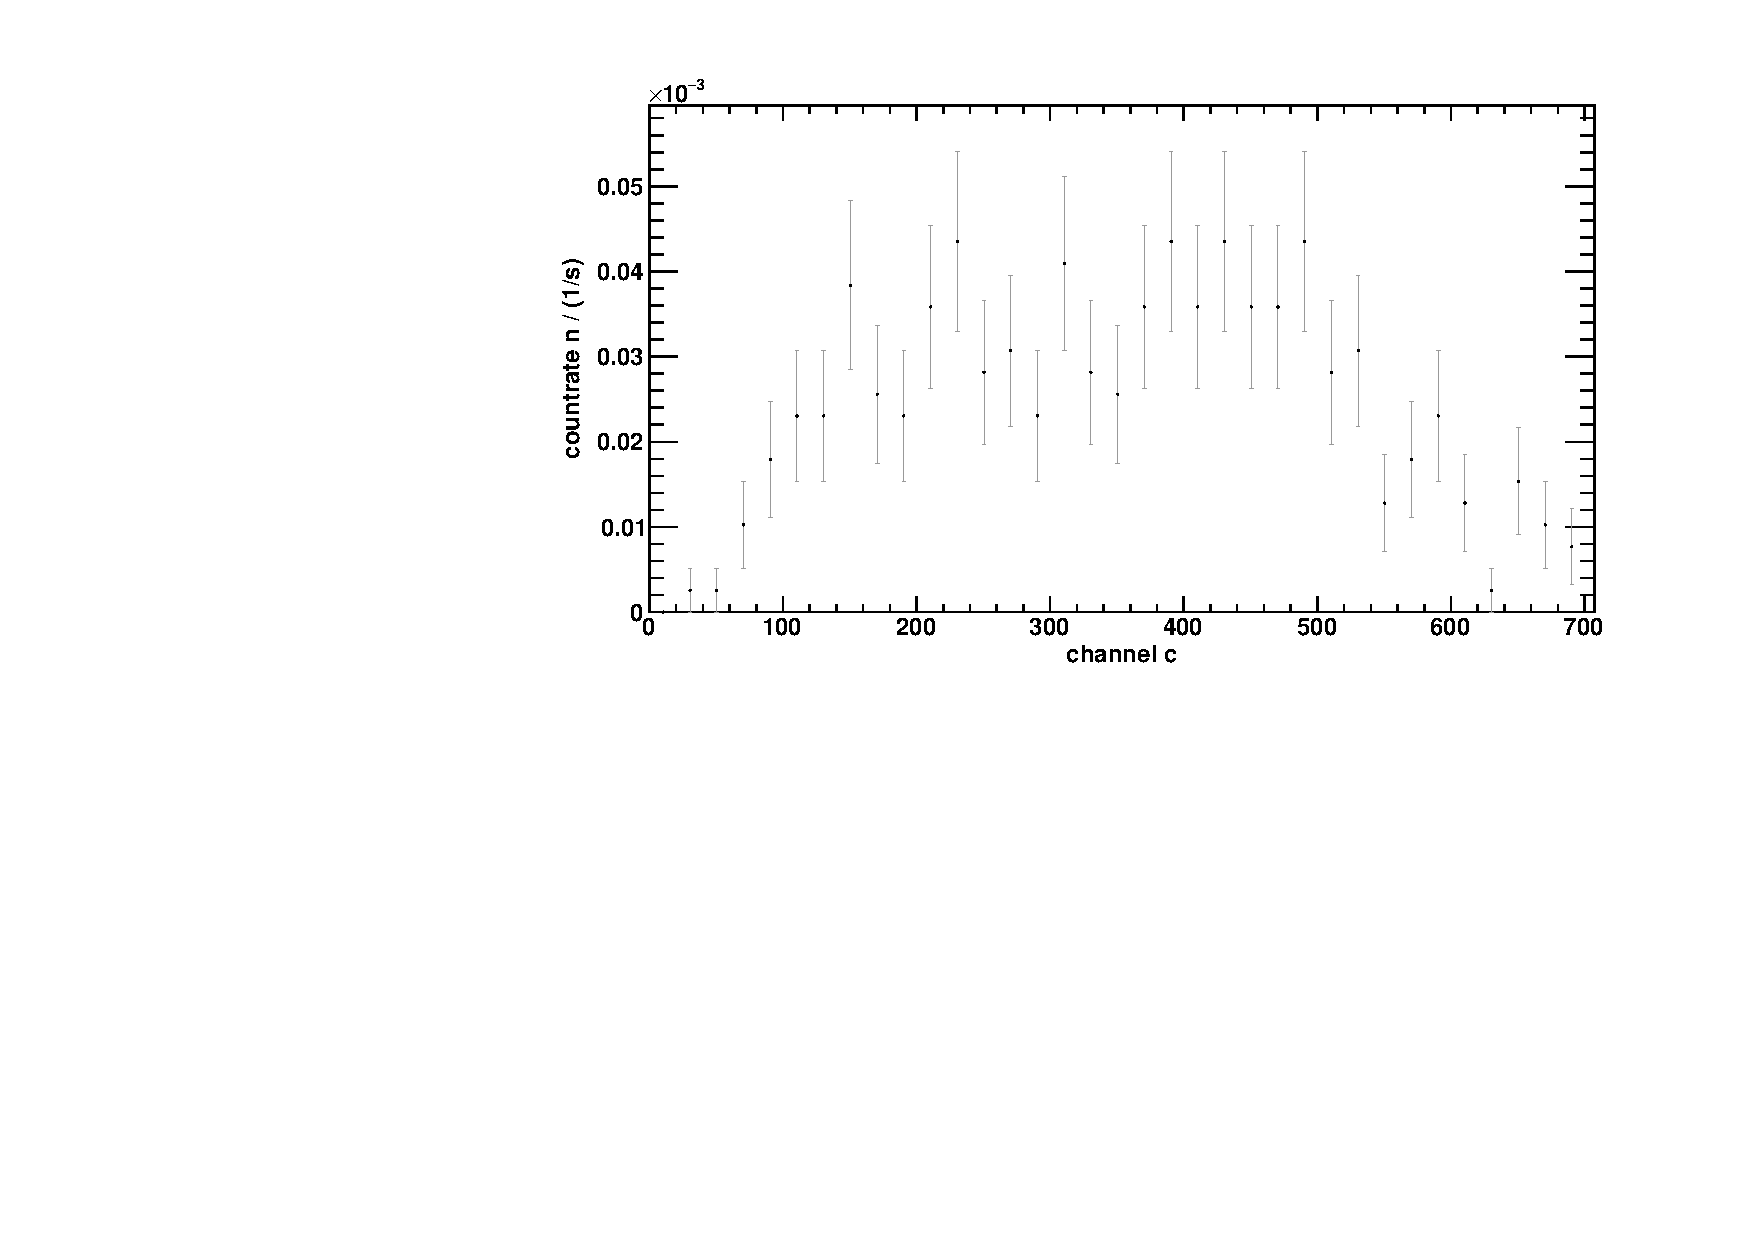
\includegraphics[width=\textwidth]{../img/underground_rebin.pdf}
  \caption{Rebinned unerground.}
  \label{img:underground:rebin}
\end{center}
\end{figure}

\subsection{\textbeta-spectrum}
The measured \textbeta-spectrum is shown in \autoref{img:beta:spectrum}.
\begin{figure}[H]
\begin{center}
  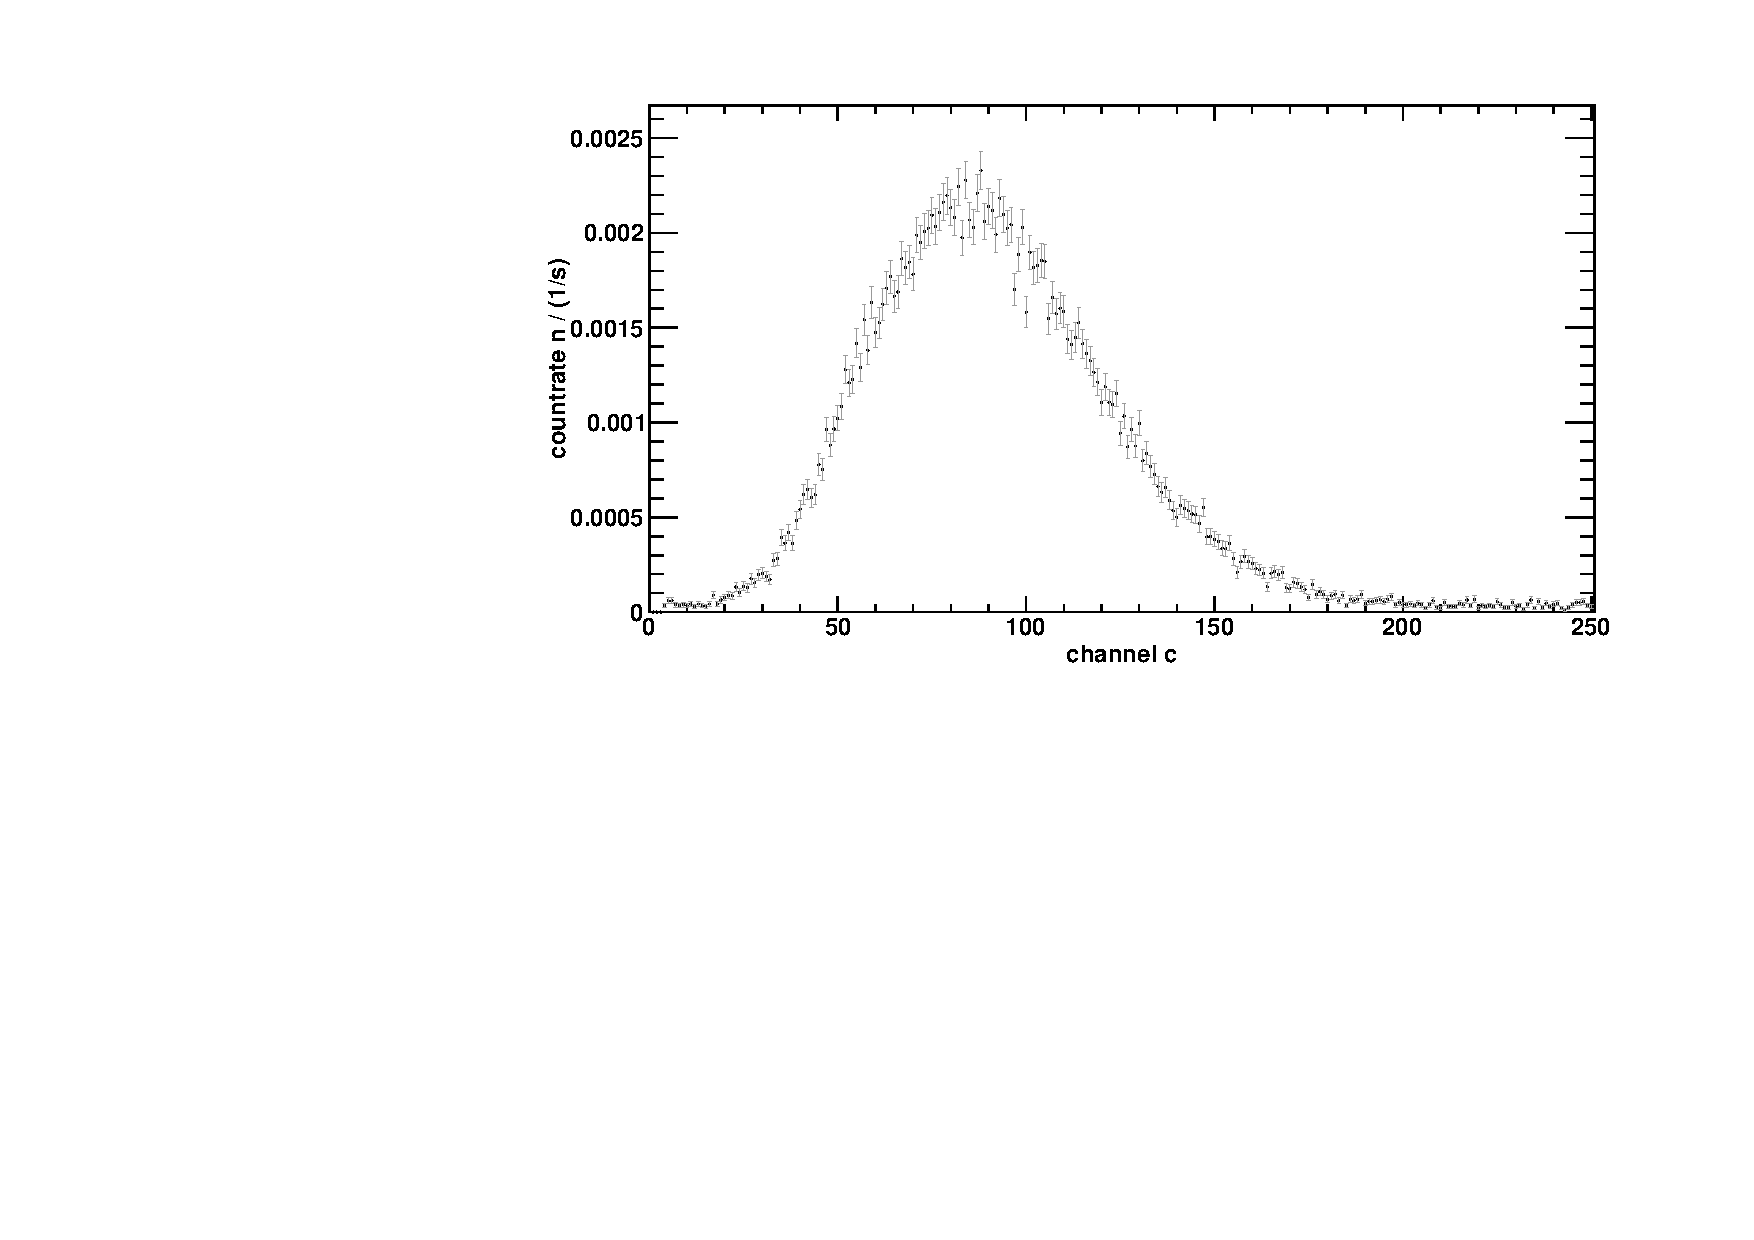
\includegraphics[width=\textwidth]{../img/betaspectrum.pdf}
  \caption{\textbeta-spectrum.}
  \label{img:beta:spectrum}
\end{center}
\end{figure}
The problem is to extract the maximal energy while taking the Gaussion blur caused by the energy resolution into account. One method is the 
\emph{Fermi-Kurie-plot} (\cite{dem4}, p.52-53).
First the channal information is converted into an energy with \autoref{eq:ecalibration}. Then $\sqrt{n(E)/E^2}$ is plotted against 
the energy $E$ (\autoref{img:beta:fermikuriefit}). Ideally a linear relationships should be identifiable. The intersection of this line with 
the $x$-axis is the maximal energy. \\
TODO warum nur teilweise linear? \\ %TODO text
The linear part gets fitted wtih
\begin{equation}
    \sqrt{n(E)/E^2} = a(E-b),
\end{equation}
so that the intersection with the $x$-axis can be read directly.
\begin{figure}[H]
\begin{center}
  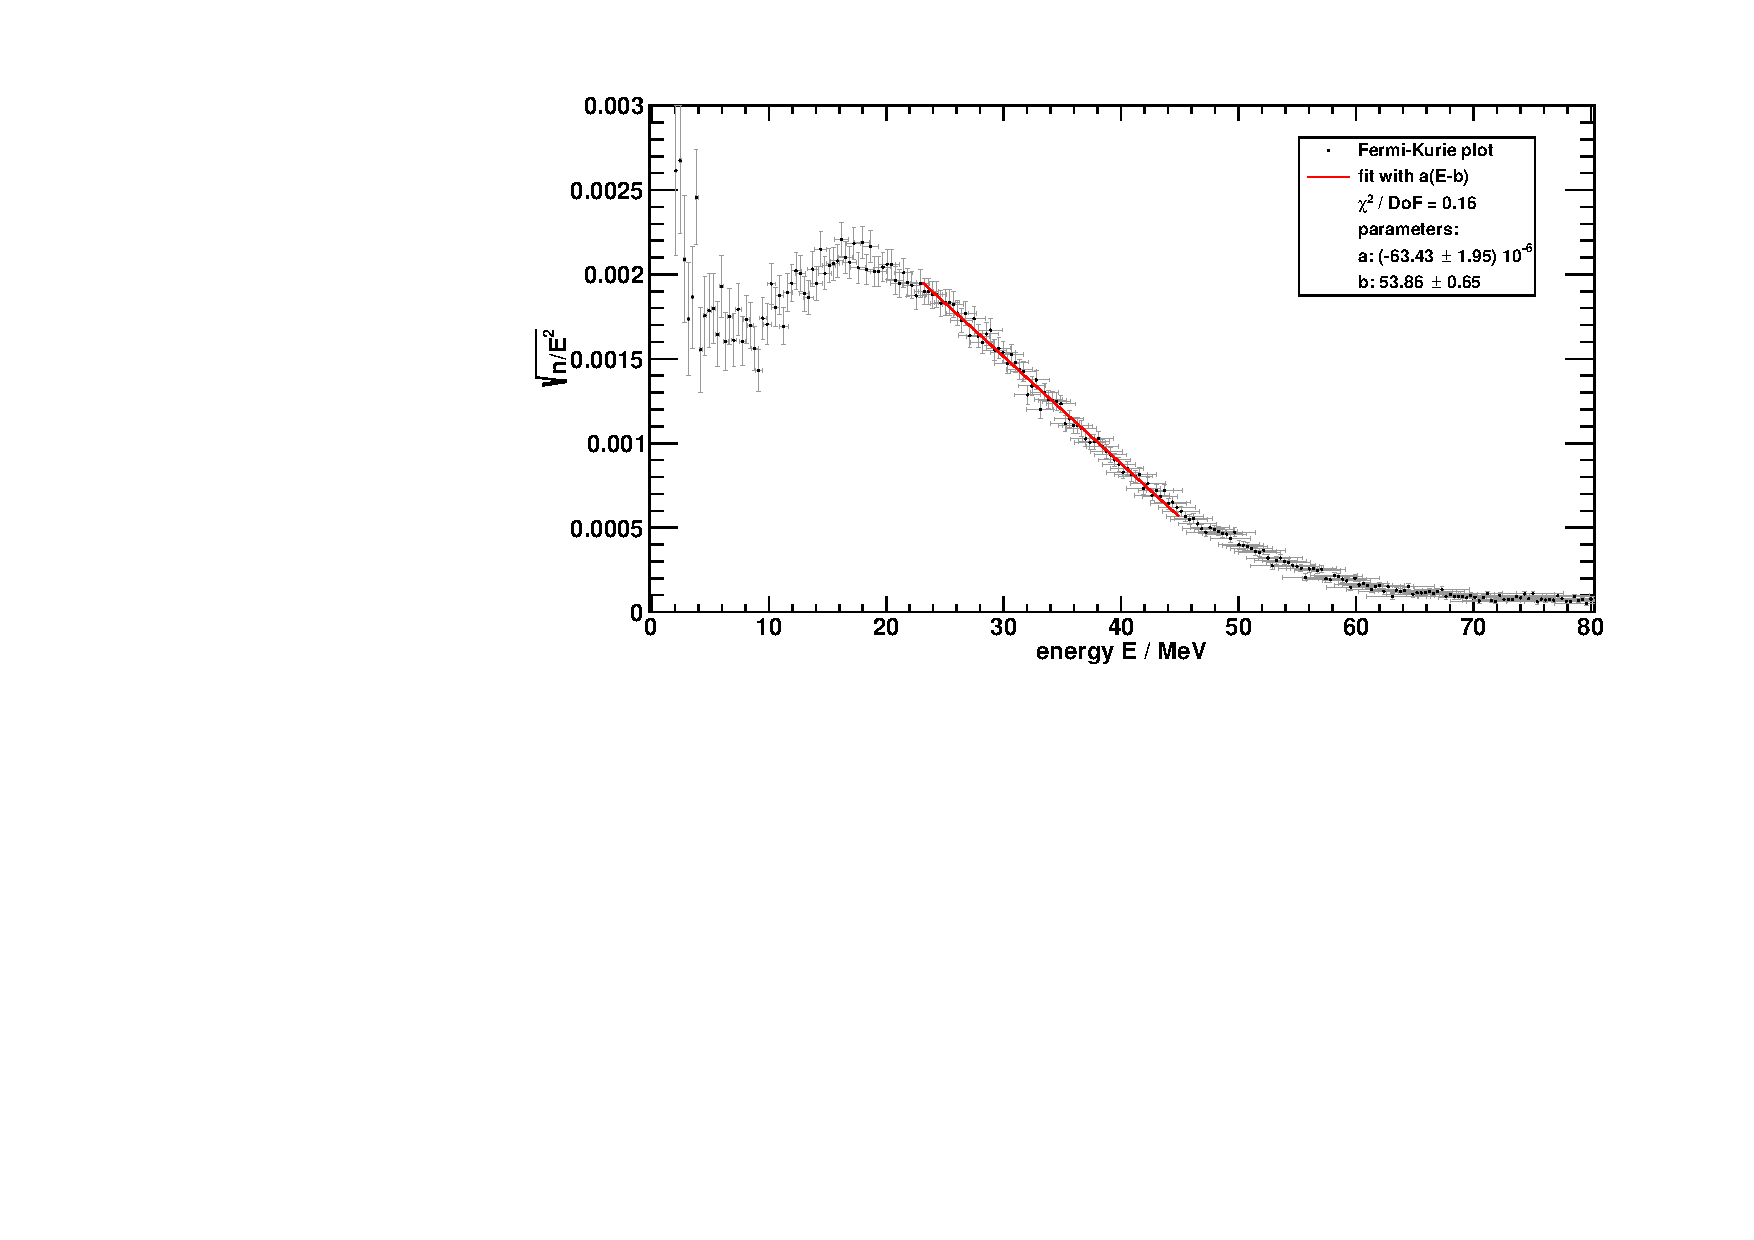
\includegraphics[width=\textwidth]{../img/betaspectrum_FermiKurie_fit.pdf}
  \caption{Fermi-Kurie plot.}
  \label{img:beta:fermikuriefit}
\end{center}
\end{figure}
With the fit one gets for $b$:
\begin{equation}
    b = (53.86 \pm 0.65)\,\text{MeV}
\end{equation}
Since this energy is half of the rest energy of the muon it has to be multiplied with 2:
\begin{equation}
\begin{split}
	\label{eq:result:mass}
    & E_\mu = 2 \cdot b, \qquad s_{E_\mu} = 2 \cdot s_b \\
    & \Rightarrow E_\mu = (107.7 \pm 1.3)\,\text{MeV}
    \end{split}
\end{equation}
The so calculated rest energy matches the literature value (\autoref{eq:litval:mass}) within a 2-\textsigma-interval.
\begin{equation}
    E_\mu^{\text{lit.}} = (105.6583715 \pm 0.0000035)\,\text{MeV}
\end{equation}

\subsection{Mean lifetime}
To calculate the mean lifetime $\tau$ of $\mu$ the channels are converted to a time with \autoref{eq:tcalibration}. 
Furthermore we rebin as described in \ref{subsub:rebinning} the spectrum to get a nicer curve. Three consecutive channels were averaged.
\begin{figure}[H]
\begin{center}
  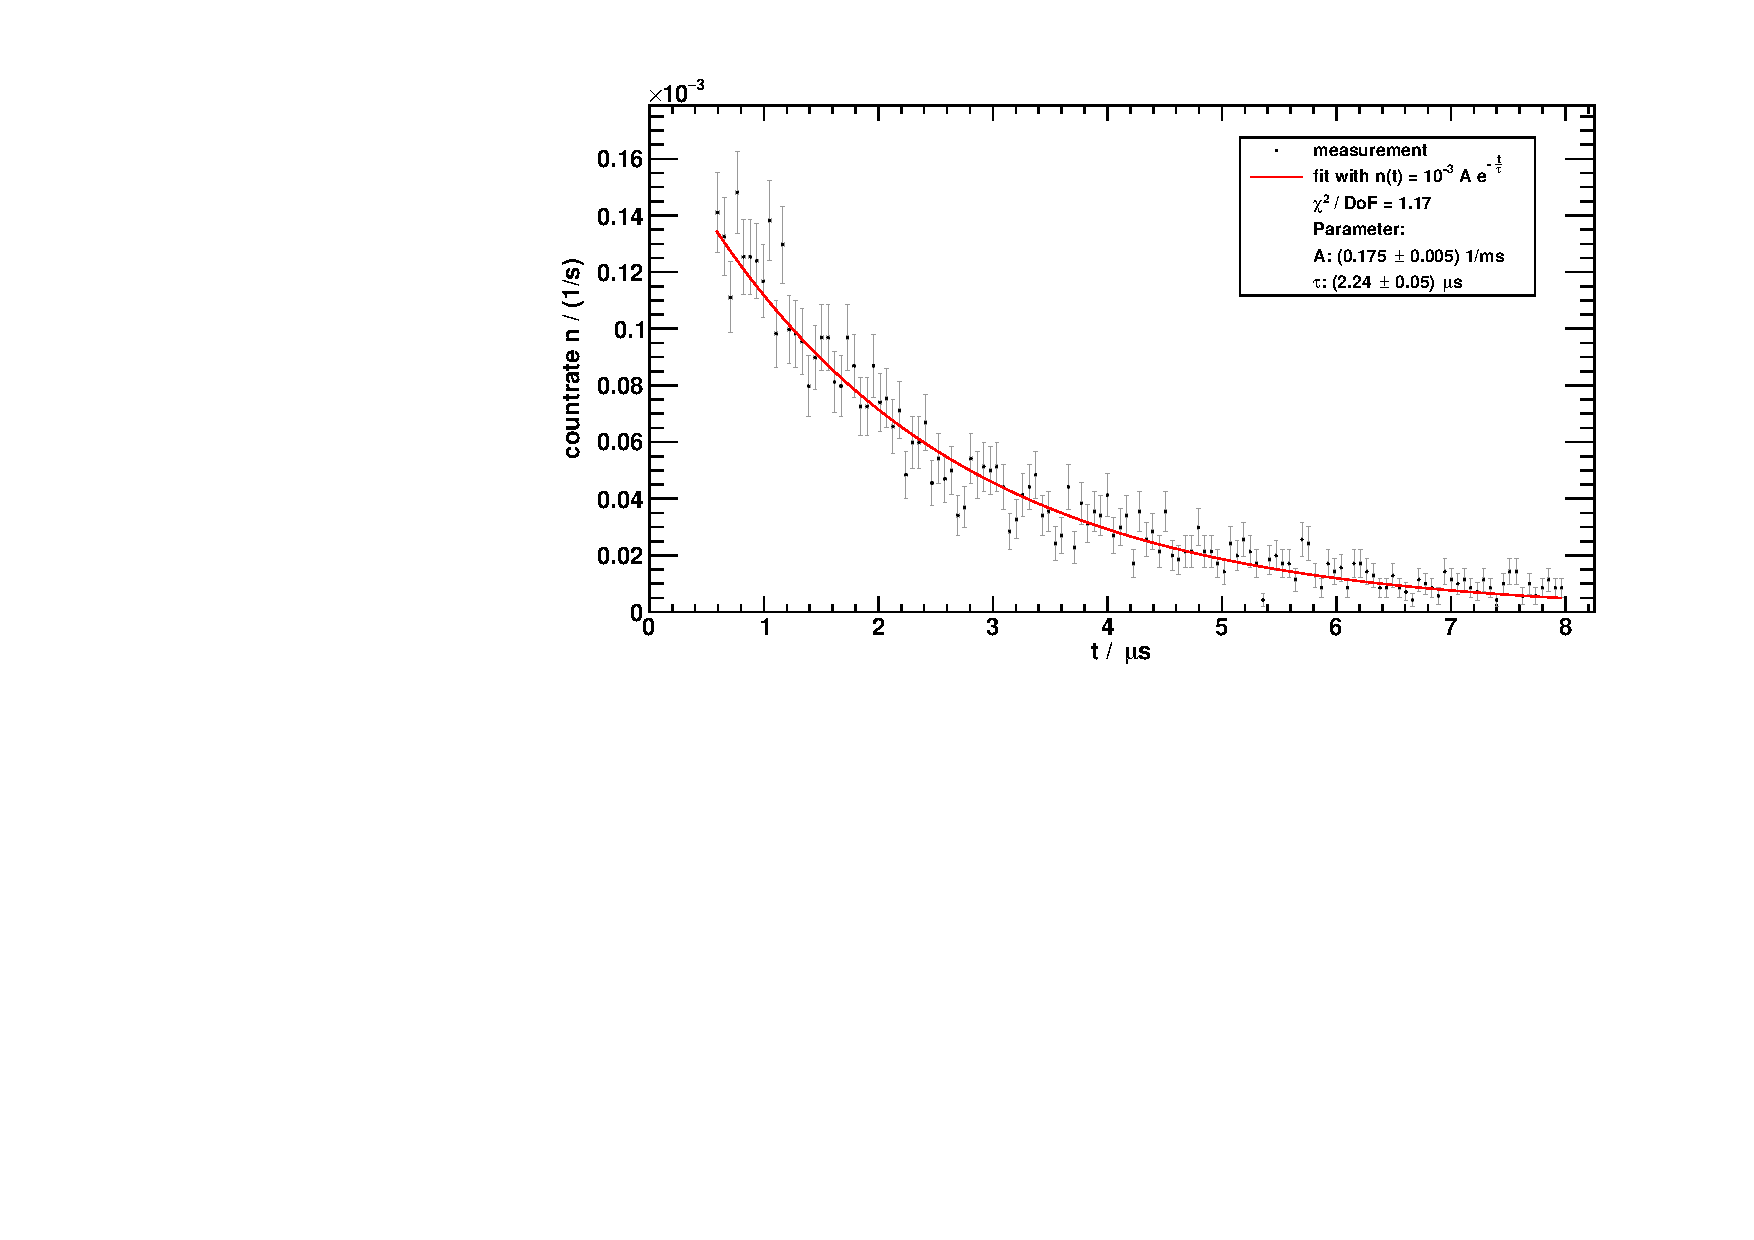
\includegraphics[width=\textwidth]{../img/decayTime.pdf}
  \caption{decay time, t-errors not visible.}
  \label{img:decaytime}
\end{center}
\end{figure}

The so obtained datapoints (\autoref{img:decaytime}) get fitted with an exponential function, since they obey the law of decay (\ref{sub:decay}):
\begin{equation}
    n = A \cdot e^{-\frac{t}{\tau}}
\end{equation}
The fit yields for the mean lifetime:
\begin{equation}
	\label{eq:result:meanlifetime}
    \tau = \left( 2.24 \pm 0.05 \right)\,\text{\textmu s}
\end{equation}
This matches with the literature value (\autoref{eq:litval:meanlifetime}) within 1-\textsigma-interval.
\begin{equation}
    \tau^{\text{lit.}} = \left( 2.1969811 \pm 0.0000022 \right)\,\text{\textmu s}
\end{equation}

\subsection{Weak coupling constant}
Now the weak coupling constant $G_\mu$ can be calculated with the muon's mass and mean lifetime. \autoref{eq:weakcouplingconstant} is used. The 
calculation is performed in natural units:
\begin{equation}
    \begin{split}
        G_\mu &= \sqrt{\frac{192 \pi^2}{\tau_\mu m_\mu^5}} \\
        s_{G_\mu} &= \frac{1}{2} \sqrt{\frac{192 \pi^3 \left( m_\mu^2 s_{\tau_\mu}^2 + 25 \tau_\mu^2 s_{m_\mu}^2 \right)}{m_\mu^7 \tau_\mu^3}}
    \end{split}
\end{equation}
With the relation
\begin{equation}
    t_\text{natural} = \frac{1}{\hbar} t_\text{S.I.}
\end{equation}
the mean lifetime can be converted to natural units. $\hbar$ has to be in eVs. \\
The weak coupling constant calculates to:
\begin{equation}
    G = (1.10 \pm 0.04) \cdot 10^{-5}\,\frac{1}{\text{GeV}^2}
\end{equation}
This result agrees with the literature value (\autoref{eq:litval:weakcouplingconstant}) within 1-\textsigma-interval.
\begin{equation}
    G_\mu^{\text{lit.}} = \left( 1.166364 \pm 0.000005 \right) \cdot 10^{-5}\,\frac{1}{\text{GeV}^2}
\end{equation}